\documentclass[10pt,a4paper]{article}
% ---------------------------------------------------------------------------

\usepackage[T1]{fontenc}
\usepackage[utf8]{inputenc}
% --- typography: Palatino text+math, Helvetica headings, txtt code ---
\usepackage[sc]{mathpazo}
\linespread{1.06}
\usepackage[scaled=0.9]{helvet}
\renewcommand{\ttdefault}{txtt}
\usepackage[protrusion=true,expansion=true]{microtype}
\usepackage[margin=2.3cm,top=2.6cm,bottom=2.6cm,headsep=0.8cm]{geometry}
\usepackage{amsmath,amssymb,amsthm}
\usepackage{booktabs,multirow,array,tabularx}
\usepackage[table]{xcolor}
\usepackage{enumitem}
\usepackage{listings}
\usepackage{tikz}
\usetikzlibrary{arrows.meta,positioning,shapes.geometric,fit,backgrounds,calc}
\usepackage{pifont}
\usepackage[strings]{underscore} % plain _ in \texttt identifiers
\usepackage{titlesec}
\usepackage{needspace}
\usepackage{etoolbox}
\usepackage{fancyhdr}
\usepackage[font=small,labelfont={bf,sf},labelsep=period,skip=5pt]{caption}
\usepackage[skins]{tcolorbox}
\usepackage{hyperref}
\usepackage[capitalise,noabbrev]{cleveref}

% --- palette ---
\definecolor{accent}{RGB}{28,62,112}
\definecolor{accentlight}{RGB}{232,238,247}
\definecolor{rawbg}{RGB}{255,248,230}
\definecolor{rawbar}{RGB}{214,150,40}
\definecolor{modelbg}{RGB}{235,244,255}
\definecolor{modelbar}{RGB}{60,110,180}
\definecolor{enginebg}{RGB}{236,250,238}
\definecolor{enginebar}{RGB}{60,145,80}
\definecolor{llmbg}{RGB}{248,238,252}
\definecolor{llmbar}{RGB}{140,80,160}

\hypersetup{colorlinks=true, linkcolor=accent, citecolor=enginebar,
  urlcolor=accent, pdftitle={When the Team Writes Itself: Composition Defects in Automatically Assembled LLM Agent Teams},
  pdfauthor={}}

% --- headings ---
\titleformat{\section}{\sffamily\Large\bfseries\color{accent}}
  {\thesection}{0.7em}{}[{\color{accent!35}\titlerule[0.6pt]}]
\titleformat{\subsection}{\sffamily\large\bfseries\color{accent}}{\thesubsection}{0.6em}{}
\titleformat{\paragraph}[runin]{\sffamily\bfseries\color{accent}}{}{0pt}{}[.]
\pretocmd{\section}{\needspace{10\baselineskip}}{}{}
\pretocmd{\subsection}{\needspace{7\baselineskip}}{}{}
\titlespacing*{\section}{0pt}{3.2ex plus 1ex minus .2ex}{1.6ex plus .2ex}
\titlespacing*{\subsection}{0pt}{2.6ex plus 1ex minus .2ex}{1.0ex plus .2ex}
\titlespacing*{\paragraph}{0pt}{1.6ex plus .5ex minus .2ex}{0.8em}

% --- header / footer ---
\pagestyle{fancy}
\fancyhf{}
\renewcommand{\sectionmark}[1]{\markboth{\thesection\quad #1}{}}
\fancyhead[L]{\sffamily\footnotesize\color{black!55}When the Team Writes Itself --- Teaching Edition}
\fancyhead[R]{\sffamily\footnotesize\color{black!55}\nouppercase{\leftmark}}
\fancyfoot[C]{\sffamily\footnotesize\color{black!60}\thepage}
\renewcommand{\headrulewidth}{0.4pt}
\renewcommand{\headrule}{{\color{black!20}\hrule width\headwidth height\headrulewidth}}
\fancypagestyle{plain}{\fancyhf{}\renewcommand{\headrulewidth}{0pt}%
  \fancyfoot[C]{\sffamily\footnotesize\color{black!60}\thepage}}

\setlist{itemsep=2pt, topsep=4pt}
\setlength{\parindent}{0pt}
\setlength{\parskip}{5pt plus 1pt}
\setlength{\emergencystretch}{3em}
\widowpenalty=10000 \clubpenalty=10000
\renewcommand{\arraystretch}{1.12}
\setlength{\tabcolsep}{5pt}

\newcommand{\cmark}{{\color{enginebar}\ding{51}}}
\newcommand{\xmark}{{\color{red!65!black}\ding{55}}}
\newcommand{\pmark}{\ding{109}}

% --- shorthands (same as the paper) ---
\newcommand{\tool}{\textsc{AgentHOT}}
\newcommand{\auto}{\textsc{AutoM2M}}
\newcommand{\Team}{\Theta}
\newcommand{\W}[1]{\textsf{W#1}}
\newcommand{\D}[1]{\textsf{D#1}}
\newcommand{\devteam}{\textsc{DevTeam}}
\newcommand{\MM}{\mathit{MM}}
\newcommand{\Mods}[1]{\mathcal{M}(#1)}
\newcommand{\TL}{\mathit{TL}}
\newcommand{\team}{\mathcal{T}}
\newcommand{\str}{\mathrm{str}}
\newcommand{\sem}{\mathrm{sem}}
\newcommand{\Dist}[1]{\mathcal{D}(#1)}
\newcommand{\fp}{\mathit{fp}}
\newcommand{\Obl}{\mathit{Obl}}
\newcommand{\cls}[1]{\textsf{#1}}
\newcommand{\code}[1]{\texttt{#1}}
\newcommand{\file}[1]{\texttt{#1}}
% robust: \tikz inside a caption (a moving argument) breaks otherwise
\DeclareRobustCommand{\tracemark}{\tikz[baseline=-0.6ex]\node[draw,diamond,fill=black!70,inner sep=1.1pt]{};}

% --- listing styles ---
\lstdefinelanguage{ATL}{
  morekeywords={module,create,from,rule,to,lazy,unique,helper,def,
                context,uses,thisModule,and,or,not,in},
  morekeywords=[2]{@llm,@check}, alsoletter={@},
  sensitive=true, morecomment=[l]{--}, morestring=[b]'}
\lstdefinelanguage{KM3}{
  morekeywords={package,class,attribute,reference,container,
                enumeration,literal,datatype,oppositeOf},
  sensitive=true, morecomment=[l]{--}}

\lstset{frame=l, framerule=2.2pt, framesep=7pt, xleftmargin=10pt,
        framexleftmargin=0pt,
        basicstyle=\ttfamily\footnotesize, breaklines=true,
        breakatwhitespace=false, columns=fullflexible, keepspaces=true,
        showstringspaces=false, numbers=none, upquote=true,
        keywordstyle=\bfseries, keywordstyle={[2]\bfseries\color{purple}},
        commentstyle=\itshape\color{black!55},
        captionpos=t, aboveskip=8pt, belowskip=8pt,
        literate={->}{{$\rightarrow$}}2 {<-}{{$\leftarrow$}}2}
% "raw input" = what the benchmark / user / lead actually provides
\lstdefinestyle{raw}{backgroundcolor=\color{rawbg}, rulecolor=\color{rawbar}, literate={}}
% "model" = a view model or metamodel as the engine holds it
\lstdefinestyle{model}{backgroundcolor=\color{modelbg}, rulecolor=\color{modelbar}}
% "engine" = deterministic output of the AgentHOT runtime
\lstdefinestyle{engine}{backgroundcolor=\color{enginebg}, rulecolor=\color{enginebar}, literate={}}
% "llm" = a prompt sent to / answer received from an LLM
\lstdefinestyle{llm}{backgroundcolor=\color{llmbg}, rulecolor=\color{llmbar}, literate={}}
\captionsetup[lstlisting]{singlelinecheck=false, margin=10pt}

% keep every listing on one page (all are short)
\BeforeBeginEnvironment{lstlisting}{\par\vspace{2pt}\noindent\begin{minipage}{\linewidth}}
\AfterEndEnvironment{lstlisting}{\end{minipage}\par\vspace{2pt}}
\crefname{lstlisting}{Listing}{Listings}
\Crefname{lstlisting}{Listing}{Listings}

% --- remarks as soft boxes ---
\newcounter{remark}
\newenvironment{remark}[1][]{%
  \refstepcounter{remark}%
  \begin{tcolorbox}[enhanced, colback=accentlight, colframe=accentlight,
      borderline west={2.2pt}{0pt}{accent}, arc=0pt, boxrule=0pt,
      left=8pt, right=8pt, top=5pt, bottom=5pt, before skip=8pt, after skip=8pt]
  \textsf{\bfseries\color{accent}Remark~\theremark\if\relax\detokenize{#1}\relax\else\ (#1)\fi.}\enspace}%
  {\end{tcolorbox}}

% A small paragraph-style marker for the "what happens" narration.
\newcommand{\what}[1]{\par\smallskip\noindent{\sffamily\bfseries\color{accent}#1}\quad}
\newcommand{\legend}[3]{\tikz[baseline=(c.base)]{\node(c)[fill=#1,inner xsep=6pt,inner ysep=2.5pt,
  font=\sffamily\footnotesize\bfseries]{\strut #3};\fill[#2](c.north west)rectangle([xshift=2.2pt]c.south west);}}


% --- teaching-edition boxes ---
\definecolor{thinkbg}{RGB}{255,246,236}
\definecolor{thinkbar}{RGB}{200,110,30}
\definecolor{keybg}{RGB}{236,247,240}
\definecolor{keybar}{RGB}{40,130,80}
\newenvironment{think}[1][Check your understanding]{%
  \begin{tcolorbox}[enhanced, colback=thinkbg, colframe=thinkbg, arc=0pt, boxrule=0pt,
     borderline west={2.2pt}{0pt}{thinkbar}, left=8pt, right=8pt, top=5pt, bottom=5pt,
     before skip=8pt, after skip=8pt]
  \textsf{\bfseries\color{thinkbar}#1.}\enspace}{\end{tcolorbox}}
\newenvironment{takeaway}{%
  \begin{tcolorbox}[enhanced, colback=keybg, colframe=keybg, arc=0pt, boxrule=0pt,
     borderline west={2.2pt}{0pt}{keybar}, left=8pt, right=8pt, top=5pt, bottom=5pt,
     before skip=8pt, after skip=8pt]
  \textsf{\bfseries\color{keybar}Key takeaways.}\par\smallskip}{\end{tcolorbox}}
\newcommand{\plain}[1]{\par\smallskip\noindent{\sffamily\bfseries\color{thinkbar}In plain words:}\enspace\emph{#1}\par\smallskip}
\begin{document}

% ---------------------------------------------------------------------------
% Title block
% ---------------------------------------------------------------------------
\thispagestyle{plain}
\begin{center}
{\sffamily\footnotesize\bfseries\color{accent}\MakeUppercase{Problem analysis and research proposal}}\par
\vspace{6pt}
{\sffamily\bfseries\fontsize{22}{26}\selectfont\color{accent}When the Team Writes Itself\par}
\vspace{6pt}
{\sffamily\large Composition Defects in Automatically Assembled LLM Agent Teams,\\
and How Model Transformations Can Check Them\par}
\vspace{10pt}
{\small\itshape Builds on ``\tool{}: M2M Transformations for Agentic
Collaborations in Software Engineering''~\cite{agenthot2026}\par}
\vspace{8pt}
{\color{accent!40}\rule{0.35\textwidth}{0.6pt}}
\end{center}
\vspace{4pt}

\begin{tcolorbox}[enhanced, colback=accentlight, colframe=accentlight, arc=0pt,
   boxrule=0pt, borderline west={2.2pt}{0pt}{accent}, left=10pt, right=10pt,
   top=7pt, bottom=7pt]
{\sffamily\bfseries\color{accent}Abstract.}\enspace
Software is increasingly built by \emph{teams} of AI agents: programs in
which a large language model (LLM) plays a role such as analyst, developer
or tester and hands its work to the next agent. Newer systems, called
\emph{team builders}, even design the team automatically for each task.
These teams fail often, and when they fail nobody can say which part was
to blame. This document argues that many of these failures have a cause
every software engineering student knows: the parts of the team have no
\emph{interfaces}. Each agent is described only by an English job
description, every hand-off is free text, and nothing checks that the
parts fit together before the team runs. We call this the
\emph{composition gap}. We support the argument with published studies,
including recent ones from ICML, ICLR, NeurIPS and ACL, and with our own
reproducible audit of 126 automatically built teams: none of their 356 job
descriptions names a teammate or says what that agent must hand over, and
in 99 of the 126 failed runs the team itself declared the task done. We
then propose \auto{}: the team builder must describe the team in a
checkable form (a \emph{typed team}), a program checks six simple rules
before the team may run, and records kept during the run point to the
exact place where something went wrong. A prototype checker catches all
82 mistakes we deliberately planted in two example teams (once the teams
declare what they must deliver, not only what they must test), finds a real
weakness in a hand-written team from earlier work, and checks a team of
1{,}000 hand-offs in a fraction of a second. We end with three research
questions and a plan to answer them. This is a \emph{teaching edition}:
it builds all the background an undergraduate in software engineering
needs, explains every idea on a running example, and ends each part with
key takeaways and questions to check your understanding.
\end{tcolorbox}

{\hypersetup{linkcolor=black}
\setcounter{tocdepth}{1}
\makeatletter
\renewcommand*\l@section[2]{\addpenalty{-\@highpenalty}\vskip 0.15em
  {\sffamily\small\@dottedtocline{1}{0em}{2em}{#1}{#2}}}
\renewcommand*\l@subsection[2]{\small\@dottedtocline{2}{2em}{2.6em}{#1}{#2}}
\makeatother
\renewcommand{\contentsname}{\sffamily\color{accent}Contents}
\tableofcontents}

% ===========================================================================
\section{How to read this document}\label{sec:read}
% ===========================================================================

\paragraph{Who this is for} An undergraduate who has taken a first
software engineering course: you know classes and interfaces, unit tests,
and UML class diagrams. You do not need to know LLMs, multi-agent systems
or model-driven engineering; \Cref{sec:course} teaches what you need.

\paragraph{The route through the document} The document has four parts.
\Cref{sec:course} is a short course on the background. \Cref{sec:plain,sec:evidence}
establish the problem: first in plain words, then with evidence.
\Cref{sec:background} explains \tool{}, the earlier work this document builds
on. \Cref{sec:rq,sec:approach,sec:checkerstudy,sec:plan} state the research
questions, explain the approach step by step, show a first prototype, and
lay out how each question will be answered. \Cref{app:glossary} is a
glossary and \Cref{app:answers} has answers to the questions in the
orange boxes.

\paragraph{Two reading paths} \emph{In 20 minutes:} read \Cref{sec:plain},
the green takeaway boxes of every section, \Cref{tab:audit}, and
\Cref{fig:w4}. \emph{In full:} read in order and answer the orange boxes
before checking \Cref{app:answers}.

\paragraph{Three kinds of boxes} Blue boxes are \emph{remarks} that sharpen
an idea. Orange boxes (``Check your understanding'') ask you a question;
try to answer before reading on. Green boxes summarise the \emph{key
takeaways} of a section.
Listings are colour-coded by where their content comes from, as in the
\tool{} companion document:

\begin{center}
\small
\begin{tabular}{@{}l p{11.5cm}@{}}
\toprule
\legend{rawbg}{rawbar}{Raw input} & Something produced outside our approach: a task, a team specification written by an existing team builder, a role prompt. \\
\legend{modelbg}{modelbar}{Model} & A metamodel, a team model or a rule module: the ``language'' and the ``sentences'' of a typed team. \\
\legend{llmbg}{llmbar}{LLM} & A prompt sent to an LLM, or the answer it returns. \\
\legend{enginebg}{enginebar}{Engine} & Deterministic output of a checker or runtime: diagnostics, trace links, reports. \\
\bottomrule
\end{tabular}
\end{center}

\paragraph{What kind of claim each statement is} Because this document
mixes published findings, our own measurements and a proposal, every
statement belongs to one of four kinds, summarised in \Cref{tab:status}. We
mark illustrative material as such where it appears.

\begin{table}[!htb]
\centering\small
\caption{Kinds of claims in this document.}
\label{tab:status}
\begin{tabularx}{\textwidth}{@{}l X l@{}}
\toprule
Kind & What it means & Where \\
\midrule
Published evidence & Numbers and findings reported by other authors, cited and paraphrased. & \Cref{sec:evidence} \\
Our measurement & A deterministic, scripted audit of public data; the script is in the artifact (\Cref{app:repro}) and reproduces every number. & \Cref{sec:audit} \\
Checker study & Output of our reference checker on typed teams and on seeded mutants; scripts and teams in the artifact. These results show that the conditions are implementable and what they catch, not that \auto{} improves task success. & \Cref{sec:checkerstudy} \\
Design & Definitions, conditions and algorithms we propose; their properties follow from the definitions. & \Cref{sec:approach} \\
Illustrative & Hand-derived examples that show how the design behaves; they are not measurements. & marked in captions \\
Planned & Studies we will run to answer the research questions, with their hypotheses and refutation criteria. & \Cref{sec:plan} \\
\bottomrule
\end{tabularx}
\end{table}

% ===========================================================================
\section{Background you need: a short course}\label{sec:course}
% ===========================================================================

This section is written for an undergraduate student who has taken an
introductory software engineering course (classes, interfaces, unit tests,
UML class diagrams) but has not studied large language models, multi-agent
systems or model-driven engineering. If you already know a topic, skip its
subsection; nothing later depends on the exercises. Every idea is tied to
an example we will reuse.

\subsection{Large language models in one page}

A \emph{large language model} (LLM) is a program that, given some text,
predicts a likely continuation. The text you give it is the \emph{prompt}.
If the prompt is ``Write a Python function that adds two numbers'', a likely
continuation is such a function. Three properties matter for this document.

\begin{itemize}
\item \textbf{It is not deterministic.} Asked twice, an LLM may answer
differently. A setting called \emph{temperature} controls how much the
answers vary; even at low temperature, small changes in the prompt can change
the answer. In software terms: an LLM is a function whose output is drawn
from a probability distribution, not computed.
\item \textbf{It can be confidently wrong.} An LLM can produce text that looks
right but is false (a ``hallucination''), for example a function that
compiles but computes the wrong thing.
\item \textbf{It only knows what is in its prompt and its training.} If an
important fact is not in the prompt, the LLM may guess it. This will matter
a lot: when one LLM passes work to another, whatever is left out of the
message is invisible to the receiver.
\end{itemize}

\subsection{From an LLM to an agent}

An \emph{agent} is an LLM wrapped in a loop with tools. The program gives the
LLM a \emph{role} (``you are a tester''), a task, and a list of tools it may
use (run code, search the web, read a file). The LLM decides on an action,
the program performs it, shows the LLM the result, and repeats until the LLM
says it is finished. So an agent is a small program whose ``brain'' is an LLM
and whose ``hands'' are tools.

\begin{lstlisting}[language=Python, style=model, caption={The agent loop, simplified (pseudocode).}, label={lst:agentloop}]
def run_agent(role, task, tools):
    history = [role, task]
    while True:
        action = llm(history)            # e.g. "run_tests()" or "DONE: ..."
        if action.startswith("DONE"):
            return action                # the agent decides it is finished
        result = tools.execute(action)   # the program performs the action
        history.append((action, result))
\end{lstlisting}

Notice the line marked \code{DONE}: the agent itself decides when it is
finished. Keep that in mind; it returns in \Cref{sec:audit}.

\subsection{Teams of agents and hand-offs}

Some tasks are too big for one agent, so several agents form a \emph{team},
much like a human software team: an analyst writes requirements, an
architect designs, a developer codes, a tester tests. When one agent's
output becomes another agent's input, we call that a \emph{hand-off}.
\Cref{fig:handoff} shows a team of four with three hand-offs.

\begin{figure}[!htb]
\centering
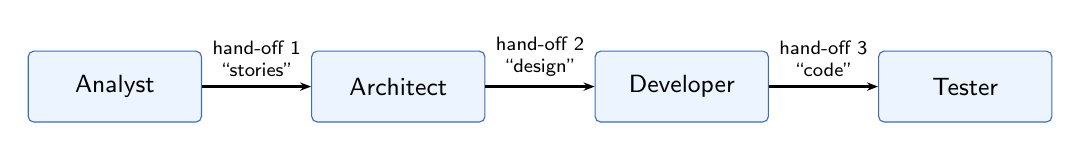
\begin{tikzpicture}[font=\sffamily\small, >={Stealth[length=4pt]},
  ag/.style={draw=modelbar, fill=modelbg, rounded corners=2pt, minimum width=22mm, minimum height=9mm, align=center},
  lbl/.style={font=\sffamily\scriptsize, align=center}]
  \node[ag] (a) at (0,0) {Analyst};
  \node[ag] (b) at (3.6,0) {Architect};
  \node[ag] (c) at (7.2,0) {Developer};
  \node[ag] (d) at (10.8,0) {Tester};
  \draw[->, thick] (a) -- node[above, lbl] {hand-off 1\\``stories''} (b);
  \draw[->, thick] (b) -- node[above, lbl] {hand-off 2\\``design''} (c);
  \draw[->, thick] (c) -- node[above, lbl] {hand-off 3\\``code''} (d);
\end{tikzpicture}
\caption{A four-agent team. Each arrow is a hand-off: one agent's output
becomes the next agent's input. In most systems today, each hand-off is a
message in English.}
\label{fig:handoff}
\end{figure}

In most of today's systems, each hand-off is just a message in English. The
Architect writes ``Here is the design: \ldots'' and the Developer's LLM reads
it and guesses what matters. Compare this with how you would connect two
classes in Java: through an \emph{interface} that the compiler checks.

\subsection{Interfaces, contracts, and why parts fail when assembled}

In a software engineering course you learn to connect components through
interfaces. An interface says what a component provides and in what form.

\begin{lstlisting}[language=Java, style=model, caption={An interface states what a component provides; the compiler checks every use.}, label={lst:java}]
interface TaskStore {
    Task create(String title);          // title must not be empty (precondition)
    Task markDone(TaskId id);           // throws if the task is already done
}
\end{lstlisting}

If a class claims to implement \code{TaskStore} but forgets \code{markDone},
the compiler refuses it \emph{before the program runs}. A \emph{contract}
goes further: it states what must hold before a call (\emph{precondition}) and
what is guaranteed after it (\emph{postcondition}). Bertrand Meyer called
this \emph{design by contract}~\cite{meyer1992dbc}.

Why bother? Because components that each work alone often fail when you put
them together. In 1995, Garlan, Allen and Ockerbloom tried to build a system
out of four well-tested, reusable components and found that the effort
exploded, because each component made hidden assumptions about the
others~\cite{garlan1995mismatch}. They called this \emph{architectural
mismatch}. Interfaces and contracts are how software engineering fights it:
they turn hidden assumptions into checked ones.

\begin{think}
In \Cref{fig:handoff}, what is the ``interface'' between the Architect and
the Developer? Who checks it? (Answer: there is none; nobody. That is the
problem this document is about.)
\end{think}

\subsection{Team builders: when an LLM designs the team}

Designing a team by hand takes effort, and a team designed for one task may
not suit another. So researchers built \emph{team builders}: an LLM (or a
program trained with machine learning) that reads a task and designs the
team for it, deciding which roles to create, what each role's prompt says,
and who talks to whom. Think of a staffing agency that, for every new
project, hires a fresh crew and writes each person a job description. The
question this document asks is: \emph{who checks that the crew fits
together?}

\subsection{Models, metamodels and transformations}

\emph{Model-driven engineering} (MDE) treats designs as structured data
that programs can check and transform. You already know its ingredients
under other names.

\begin{itemize}
\item A \textbf{metamodel} is a description of what may be said: a class
diagram, a database schema, or a JSON Schema. It says, for example, ``a
\cls{UserStory} has a title and one or more \cls{Criterion} objects''.
\item A \textbf{model} is data that follows the metamodel: the rows of the
database, or a JSON document that validates against the schema. We say the
model \emph{conforms} to the metamodel.
\item A \textbf{transformation} is a program that reads models of one
metamodel and writes models of another, by \emph{rules} such as ``for every
\cls{UserStory}, create one API \cls{Operation}''. ATL is a well-known
language for writing such rules~\cite{jouault2008atl}.
\item A \textbf{trace link} is a record the transformation keeps: ``this
operation was created from that story by that rule''. Trace links let you
answer ``if this story changes, what else must change?''.
\end{itemize}

\begin{remark}[An analogy we will use throughout]
A metamodel is a \emph{form}; a model is a \emph{filled-in form}; a
transformation is a clerk who reads one filled-in form and fills in
another, following written rules; a trace link is the clerk's note ``I
filled box 7 of form B from box 3 of form A''.
\end{remark}

\paragraph{Navigating models with OCL} Rules need to say things like
``the titles of this story's criteria''. MDE uses a small expression
language, OCL, for that. You can read an OCL path exactly like a chain of
field accesses in Java: \code{s.criteria.text} means ``take story
\code{s}, follow its \code{criteria} link, and read each criterion's
\code{text}''. A \emph{guard} such as \code{s.status = 'accepted'} is a
boolean condition, like the condition of an \code{if}. That is all the OCL
you need for this document.

\subsection{Static versus dynamic checking}

A \emph{static} check examines a program without running it; the Java
compiler's type check is static. A \emph{dynamic} check runs the program,
as a unit test does. Static checks are cheap and catch whole classes of
mistakes before anything runs; dynamic checks catch what static checks
cannot see. The approach in this document adds a static check for
\emph{teams} and keeps dynamic checks (tests) for the values the agents
produce.

\subsection{Graphs and reachability}

A \emph{graph} is a set of nodes connected by arrows. ``Is node $B$
\emph{reachable} from node $A$?'' means: can you follow arrows from $A$ and
arrive at $B$? A program answers this with a breadth-first or depth-first
search in time proportional to the size of the graph. Several of our checks
are reachability questions, for example: ``does every requirement reach a
test?''

\subsection{Oracles, validators and mutation testing}

A \emph{test oracle} decides whether an output is correct, such as
\code{assert add(2,3) == 5}. In this document a \emph{validator} is any
automatic check that a value must pass before it is accepted; some only
check \emph{form} (``does it parse?''), others check \emph{behaviour} (``does
the code pass the tests?''). \emph{Mutation testing} evaluates a checker by
deliberately injecting small mistakes (\emph{mutants}) and counting how many
the checker catches; a caught mutant is said to be \emph{killed}. We use
mutation testing to evaluate our team checker in \Cref{sec:checkerstudy}.

\subsection{How team builders learn: two terms}

Some recent team builders are trained with \emph{reinforcement learning}
(RL): the builder tries a team, the team attempts the task, and the builder
receives a numerical \emph{reward} (for example 1 if the answer was right,
0 otherwise), which it learns to increase over many attempts. Others use a
\emph{graph neural network} (GNN), a machine-learning model that takes a
graph (here, agents and who talks to whom) as input and learns to produce
a good graph for a task. You do not need the mathematics of either; what
matters is that both learn only from the final reward or score.

\subsection{How a research paper argues}

A research paper states \emph{research questions} (RQs), explains how it
will answer each one, and lists \emph{threats to validity}: reasons its
conclusions might be wrong. A good paper also says what result would
\emph{refute} its claim. Two statistical terms appear in our plan: a
\emph{bootstrap confidence interval} estimates the uncertainty of a
measured share by re-sampling the data many times, and \emph{Cohen's
$\kappa$} measures how much two people who label the same data agree beyond
chance (1 means perfect agreement, 0 means chance level). You will find all of these in
\Cref{sec:rq,sec:plan}.

\begin{takeaway}
\begin{itemize}
\item An LLM is a non-deterministic text predictor; an agent is an LLM in a
loop with tools; a team is several agents passing work through hand-offs.
\item In today's teams, hand-offs are English messages with no interface and
no checker.
\item Software engineering fights ``parts that don't fit'' with interfaces,
contracts and static checks; MDE gives us forms (metamodels), filled-in forms
(models), rules (transformations) and records (trace links).
\end{itemize}
\end{takeaway}

% ===========================================================================
\section{The problem in plain words}\label{sec:plain}
% ===========================================================================

\subsection{From hand-designed teams to teams that write themselves}

Large language models (LLMs) are increasingly used as \emph{agents}: a
program gives an LLM a role (``you are a tester''), some tools (a code
runner, a web search), and a task, and lets it act. Several agents can form
a \emph{team}. Early teams for software engineering were designed by hand:
MetaGPT and ChatDev fix a product manager, an architect, an engineer and a
tester, and the order in which they pass work to each
other~\cite{hong2024metagpt,qian2024chatdev,dong2024selfcollab}. A recent
literature review in TOSEM describes this design space and its open
problems for software engineering~\cite{he2025lma}.

Hand-designed teams do not adapt to new tasks, so a second generation of
systems builds the team \emph{automatically}. We call such a system a
\emph{team builder}. Given a task, a team builder decides which agents to
create, writes each agent's role description, and decides who talks to
whom. Examples include CaptainAgent~\cite{song2024captain},
AutoAgents~\cite{chen2024autoagents}, AgentVerse's expert
recruitment~\cite{chen2024agentverse}, DyLAN~\cite{liu2024dylan},
EvoAgent~\cite{yuan2025evoagent}, MetaAgent~\cite{zhang2025metaagent} and
MAS-Zero~\cite{ke2025maszero}; a neighbouring line searches over agentic
workflows and topologies offline (ADAS, AFlow, GPTSwarm,
MaAS)~\cite{hu2025adas,zhang2025aflow,zhuge2024gptswarm,zhang2025maas}.
\Cref{lst:captain} shows, verbatim, part of what one team builder actually
produced for one task.

\begin{lstlisting}[style=raw, caption={Raw input: a team specification produced by CaptainAgent for one GAIA task (Who\&When, Algorithm-Generated, file \file{1.json}; role prompts abridged, plan verbatim).}, label={lst:captain}]
Team: Excel_Expert, BusinessLogic_Expert, DataVerification_Expert (+ Computer_terminal)

Excel_Expert: "Expert in analyzing and processing data from Excel files.
  You will be responsible for scrutinizing, interpreting, and managing data
  from Excel files ... pivot tables, data visualization, data cleaning ..."
BusinessLogic_Expert: "... comprehending complex business requirements and
  translating them into actionable data logic ..."
DataVerification_Expert: "... employing Bing Search API ... vigilantly
  verifying the accuracy of this information ..."

## Plan for solving the task                     (manager brief, shared)
1. Load the provided Excel file and read the client data.
2. Identify the street addresses of the clients.
3. Determine which addresses are even-numbered (facing west).
4. Count the number of clients with even-numbered addresses ...
## Output format
The number of clients receiving the sunset awning design.
\end{lstlisting}

Read \Cref{lst:captain} as a software engineer would read an architecture
document. Each role says what the agent is \emph{good at}. None says what
the agent \emph{receives}, what it must \emph{produce}, in what form, or
\emph{for whom}. The plan lists four steps but does not say which agent
performs which step. The only output format is for the whole team. Whether
the street-number parsing in step~3 is the Excel expert's job or the
business-logic expert's, and who checks it, is left to the agents to work
out while they talk. In this run, the annotators of the benchmark attribute
the failure to the Excel expert, whose code mishandled street-address edge
cases; the verification expert declared the result verified, and the team
terminated with a wrong answer.

\subsection{The composition gap}

A team builder is an architect that composes a system out of components (the
agents) and connectors (the hand-offs between them). In software
architecture this situation has a name. Garlan, Allen and Ockerbloom showed
that components that are individually sound fail when they are assembled,
because each embodies implicit assumptions about the others that nobody
checks: \emph{architectural mismatch}~\cite{garlan1995mismatch}. Fourteen
years later they found the problem still largely
unsolved~\cite{garlan2009mismatch}. The classic remedies make the
assumptions explicit and checkable: typed interfaces and contracts on what
each component requires and ensures~\cite{meyer1992dbc}, and formal
connector specifications that can be checked for
compatibility~\cite{allen1997connection}.

An automatically assembled team of LLM agents has no such interfaces. Every
agent is specified in prose, every hand-off is free text that the next LLM
re-interprets, and the assembled team is executed without any check that its
parts fit. We call this the \emph{composition gap}:

\begin{remark}[The composition gap]
A team builder produces a team whose agents' inputs, outputs, ownership of
work, and completion criteria are stated only in natural language, so no
property of how the agents fit together is checked before or during
execution. Failures caused by the composition therefore surface only as
end-to-end task failures, and cannot be told apart from failures of an
individual agent.
\end{remark}

The gap is sharper for automatically assembled teams than for hand-designed
ones for three reasons. First, there is no human architect who reviews the
composition: the team exists only for one task. Second, the builders are
evaluated and optimised on end-to-end task scores, so a composition defect
and an agent's reasoning error look the same to the optimiser
(\Cref{sec:ev-builders}). Third, when the team fails, the only artefact is a
transcript, and attributing the failure to a component is hard even for
the strongest models (\Cref{sec:ev-attrib}).

\begin{tcolorbox}[enhanced, colback=accentlight, colframe=accentlight, arc=0pt,
   boxrule=0pt, borderline west={2.2pt}{0pt}{accent}, left=10pt, right=10pt,
   top=6pt, bottom=6pt]
{\sffamily\bfseries\color{accent}In one sentence.}\enspace Team builders
compose agents whose interfaces are prose, so composition defects are
neither prevented, nor detected, nor attributable; \Cref{sec:statement}
states this precisely after the evidence.
\end{tcolorbox}

\Cref{sec:evidence} turns this argument into evidence. \Cref{sec:background}
then explains \tool{}, which closes the gap for \emph{hand-written} teams,
and \Cref{sec:approach} extends it to teams that write themselves.
% ===========================================================================
\section{Evidence: why automatically assembled teams fail}\label{sec:evidence}
% ===========================================================================

This section collects the evidence in five steps: teams fail at the seams
between agents (\Cref{sec:ev-seams}); team builders do not check those seams
(\Cref{sec:ev-builders}); failures of assembled teams are hard to attribute
(\Cref{sec:ev-attrib}); the team specifications themselves contain no
interfaces (\Cref{sec:audit}); and software engineering and multi-agent
research have long-standing names for this problem (\Cref{sec:ev-names}).
\Cref{sec:statement} condenses the evidence into a problem statement.

\subsection{Multi-agent teams fail at the seams}\label{sec:ev-seams}

\paragraph{MAST} Cemri et al.\ (NeurIPS 2025) built MAST-Data, more than
1{,}600 annotated traces from seven multi-agent frameworks including
MetaGPT, ChatDev, AG2 and Magentic-One, and derived a taxonomy of 14
failure modes from expert annotation with high inter-annotator
agreement~\cite{cemri2025mast}. They report that the performance gains of
multi-agent systems over single agents on popular benchmarks are often
minimal. In their taxonomy, 44.2\% of failure occurrences are \emph{system
design issues} and 32.3\% \emph{inter-agent misalignment}; the remainder
concern \emph{task verification}. In other words, about three quarters of
the failures they observe concern how the team is put together and how its
members exchange work, not what a single model knows.

\paragraph{Edge-level errors} Lin et al.\ (ACL 2026) audited execution logs
of multi-agent systems and located the failures on the \emph{edges} of the
team, the hand-offs~\cite{lin2026agentask}. Their taxonomy has four types:
a \emph{data gap} (a message lacks details the receiver needs),
\emph{signal corruption} (a malformed or distorted intermediate result is
passed on as fact), \emph{referential drift} (an ambiguous reference is
interpreted differently downstream), and a \emph{capability gap} (a
sub-task is sent to an agent that cannot perform it). They attribute the
failure of multi-agent systems to beat strong single agents consistently
to errors that propagate through such hand-offs.

\paragraph{Teams do not use the expertise they have} Pappu et al.\
(ICML 2026) studied teams of LLM agents that organise themselves, and gave
one member the knowledge needed to solve the task~\cite{pappu2026experts}.
Unlike human teams in comparable experiments, the LLM teams consistently
failed to match the performance of their expert member, even when they
were told explicitly who the expert was. The bottleneck was not finding
the expert but \emph{using} the expert: the agents tended to average the
expert's view with everyone else's, a tendency that grew with team size.

\paragraph{Talking is not the same as coordinating} SILO-BENCH (ACL 2026)
gives each agent only a fragment of an algorithmic problem with an exact
answer, so the agents must combine their information~\cite{zhang2026silobench}.
Across 1{,}620 experiments, agents communicated actively yet failed to turn
the communication into a correct joint computation, which the authors call
a \emph{communication--reasoning gap}. MultiAgentBench (ACL 2025) likewise
measures the quality of collaboration, not only task success, and finds that
the choice of coordination topology changes results~\cite{zhu2025multiagentbench};
Riedl (ICLR 2026) shows that higher-order coordination among LLM agents can
be steered by prompt design but does not appear by
itself~\cite{riedl2026emergent}.

\paragraph{Controlled scaling studies} Kim et al.\ ran a controlled
evaluation of single-agent and four multi-agent architectures across
several benchmarks and LLM families, holding tools, prompts and budgets
fixed~\cite{kim2025scaling}. Relative to a single agent, multi-agent
performance ranged from roughly $+81\%$ on decomposable tasks to $-70\%$ on
sequential planning, and architectures without a central verification
point propagated errors more. Whether a team helps depends on whether its
structure fits the task, which is exactly what a team builder decides.

\paragraph{Software-engineering venues} Lu, Li and Huo (ASE 2025) built 34
programmable tasks and found that three popular agent frameworks with two
LLM backbones completed only about half of them; their failure taxonomy
highlights planning errors, task-execution issues and incorrect responses,
and they note that evaluations rarely analyse the communication between
agents~\cite{lu2025exploring}. He, Treude and Lo's TOSEM review surveys
LLM-based multi-agent systems for software engineering and sets out a road
map for them~\cite{he2025lma}, and Liu et al.'s TOSEM survey of LLM-based
agents for software engineering describes multi-agent teams that mimic
human development roles~\cite{liu2024agents4se}.
From the multi-agent-systems community, La Malfa et al.\ (NeurIPS 2025
position track) argue that LLM-based ``multi-agent systems'' largely
ignore the coordination and communication protocols that classical
multi-agent research developed, and rely on ambiguous natural-language
exchange instead~\cite{lamalfa2025miss}.

\subsection{Team builders optimise what they can measure}\label{sec:ev-builders}

\Cref{tab:builders} summarises, to our reading of each paper, what
sixteen team builders and workflow designers generate and what they check before or after running the
team. The pattern is consistent. Every builder generates roles and, in most
cases, a topology or workflow. The quality signal is either an end-to-end
score on a validation set, the judgement of another LLM (a critic, observer,
filter or verifier), or execution feedback from the task. None of them
states, for each pair of agents, what is handed over and in what form, and
none checks such a statement before running the team. MetaAgent comes
closest: its finite state machine makes \emph{control} explicit (which agent
acts in which state, and when the system moves back to an earlier
state)~\cite{zhang2025metaagent}, but the content passed between states
remains free text. MAS-Zero adds meta-level feedback on whether a design is
solvable and complete~\cite{ke2025maszero}; that feedback is itself an LLM
judgement.

\begin{table}[!htb]
\centering\small
\caption{What team builders generate and what they check (our reading of each paper).}
\label{tab:builders}
\rowcolors{2}{black!3}{white}
\begin{tabularx}{\textwidth}{@{}l X X X@{}}
\toprule
\rowcolor{white}Builder & Generates & Quality signal & Hand-off contract checked? \\
\midrule
CaptainAgent~\cite{song2024captain} & roles, prompts, tools per sub-task & filter LLM selects agents; reflector LLM reviews nested chat & no \\
AutoAgents~\cite{chen2024autoagents} & agent team and execution plan & observer LLM reflects on plan and agents & no \\
AgentVerse~\cite{chen2024agentverse} & recruited experts & evaluator feedback after execution & no \\
DyLAN~\cite{liu2024dylan} & agent selection in a dynamic network & unsupervised agent-importance score & no \\
EvoAgent~\cite{yuan2025evoagent} & agent variants by mutation/crossover & evolutionary selection on task results & no \\
MetaAgent~\cite{zhang2025metaagent} & finite-state-machine team & optimisation after design & control only, not content \\
MAS-Zero~\cite{ke2025maszero} & per-instance team designs & LLM meta-feedback, verifier & no (LLM-judged completeness) \\
ADAS, AFlow, MaAS~\cite{hu2025adas,zhang2025aflow,zhang2025maas} & agentic workflows as code/graphs & score on a validation set & no \\
G-Designer~\cite{zhang2025gdesigner} & communication topology (graph neural network) & task performance and token cost & no \\
Puppeteer~\cite{dang2025puppeteer} & which agent acts next (RL-trained orchestrator) & task reward & no \\
Conductor~\cite{nielsen2026conductor} & natural-language workflow: sub-tasks, agents, visibility & task reward plus a parse-only format reward & form of the plan only \\
AgentNet~\cite{yang2025agentnet} & decentralised, evolving agent graph & task feedback & no \\
MAS-Orchestra~\cite{ke2026masorchestra} & whole team at once (RL, function calls) & task reward & no \\
ANN~\cite{ma2026ann} & layered teams refined by textual feedback & task feedback & no \\
\bottomrule
\end{tabularx}
\end{table}

The most recent builders make the point sharper, not weaker. They learn
to build teams with reinforcement learning, so the only teacher is the
final reward: the Conductor writes its whole workflow in natural language
and is rewarded for task success plus a reward for producing a parseable
plan~\cite{nielsen2026conductor}; the Puppeteer learns which agent should
act next~\cite{dang2025puppeteer}; MAS-Orchestra generates an entire team
at once and opens by observing that automatic team design still
under-delivers~\cite{ke2026masorchestra}. A parseable plan is a checked
\emph{form}; nobody checks that the plan's parts \emph{fit}.

Two consequences follow. First, a composition defect is only ever observed
through a lower task score, together with every other source of error, so
the optimiser cannot learn \emph{which} part of the composition was wrong.
Recent self-improving builders try to recover this information from
traces as ``textual gradients''~\cite{he2026tpgo}; they read it back from
prose. Second, the signal that a builder uses to repair a team is often
another LLM's opinion of a transcript, which inherits the attribution
problem of the next subsection.

\subsection{Failures of assembled teams are hard to attribute}\label{sec:ev-attrib}

\paragraph{Who\&When} Zhang et al.\ (ICML 2025) collected failure logs from
127 multi-agent systems, most of them generated automatically by the
CaptainAgent team builder on GAIA and AssistantBench tasks, plus the
hand-crafted Magentic-One~\cite{zhang2025whowhen}. Human annotators marked,
for each failure, the responsible agent, the decisive step, and a reason.
The best automated attribution method identified the responsible agent in
53.5\% of cases and the decisive step in only 14.2\%; some methods
performed below random, and strong reasoning models did not reach
practical usability.

\paragraph{TraceElephant} Chen et al.\ re-ran CaptainAgent, Magentic-One and
SWE-Agent with complete inputs recorded~\cite{chen2026traceelephant}.
Full traces helped, but average attribution accuracy remained around
two thirds for agents and below one third for steps. Two of their findings
bear directly on our problem. In the automatically assembled team
(CaptainAgent) decisive failure steps were dispersed over the whole run,
because errors can enter during agent selection, planning, coordination or
tool use; in the hand-crafted systems they concentrated early.
Orchestrator and planner agents caused a non-negligible share of failures
(18--29\%), through incorrect decomposition, sub-optimal agent selection
or flawed coordination. And attribution needed the \emph{input} side of
each step, because only the input shows whether an agent failed by itself
or received missing or transformed information from upstream.

That last observation is the hinge of this document. In a free-text team,
what an agent received is a conversation prefix of unbounded size. In
\tool{} (\Cref{sec:background}), what an LLM received for one value is a
declared, bounded \emph{footprint}, recorded with a digest. The information
that attribution needs is therefore present by construction.

\subsection{Our audit: team specifications without interfaces}\label{sec:audit}

The Who\&When repository publishes, for each of its 126 automatically
assembled failing teams, the role prompt that CaptainAgent generated for
every agent and the manager's brief that opens the run. These are the
complete specifications of the teams. We audited them with a deterministic
script (\Cref{app:repro}) that asks only what the specification
\emph{states}, not how the agents behaved. \Cref{tab:audit} gives the
results.

\begin{table}[!htb]
\centering\small
\caption{Structural audit of the 126 automatically assembled teams in Who\&When
(Algorithm-Generated split; 356 generated roles). All counts reproduced by
\file{audit_whowhen.py}; every lexical match was inspected by hand.}
\label{tab:audit}
\begin{tabularx}{\textwidth}{@{}X r r@{}}
\toprule
Question asked of the team specification & Count & Share \\
\midrule
Roles whose prompt names any teammate & 0 / 356 & 0.0\% \\
Roles whose prompt states what the role must output & 0 / 356 & 0.0\% \\
Roles with any hand-off-like phrase (deliberately loose pattern) & 27 / 356 & 7.6\% \\
\quad of which: templated ``validate the answers derived by your colleagues'' & 16 & \\
\quad of which: generic mention of ``teammates'' or ``other team members'' & 3 & \\
Teams whose plan assigns any step to a named role & 0 / 126 & 0.0\% \\
Teams with an output format (for the whole team only) & 126 / 126 & 100.0\% \\
Teams with at least one role named as verifier or validator & 100 / 126 & 79.4\% \\
\midrule
Failed runs that ended with an agent declaring \code{TERMINATE} & 99 / 126 & 78.6\% \\
\quad of which the terminating agent was a verifier/validator role & 42 / 126 & 33.3\% \\
Runs in which the annotated mistake agent is a verifier/validator role & 29 / 126 & 23.0\% \\
\bottomrule
\end{tabularx}
\end{table}

The first block concerns the specification. Not one of the 356 generated
roles names a teammate or states what it must produce. Under a deliberately
loose pattern for hand-off language, 27 roles match; on inspection, 16 are
copies of one templated validator prompt that refers to ``answers derived
by your colleagues'' without saying which colleague or what form the answer
takes, 3 mention teammates generically, and the remaining 8 are false
positives (for example, ``clients receive advice''). Every team has a plan,
and no plan step names the role that performs it. The only interface the
specification states is the format of the team's final answer.

The second block concerns how these runs ended. Who\&When contains only
failed runs, so these numbers do not compare failing with succeeding teams.
What they show is how the failures \emph{ended}: in 99 of the 126 runs an
agent declared the task complete, 42 times a role whose name says it
verifies or validates, rather than the run stopping without such a
declaration. These failures were not detected by the team that produced
them. In 29 runs, the annotators name a verification role as the agent
that made the decisive mistake. Termination in these teams is a claim made
in the conversation, not a property that anything checks.

\paragraph{An objection: shared context makes interfaces unnecessary}
CaptainAgent's teams talk in a group chat in which every agent sees every
message, a blackboard design. One could argue that explicit hand-offs are
unnecessary there, and that \Cref{tab:audit} measures a paradigm rather
than a defect. We take the objection seriously and answer it in three
ways. First, a shared transcript removes the \emph{transport} problem, not
the \emph{ownership} problem: who performs plan step~3, and who checks it,
is still unspecified (\D{1}, \D{3}). Second, the failure modes that MAST
attributes to unstructured shared conversation (loss of history,
conversation reset, ignored input, information withholding) are failures
\emph{of} shared context~\cite{cemri2025mast}. Third, a contrast with the
hand-crafted system in the same benchmark: \Cref{tab:contrast} counts, at
runtime, the agent messages whose content names another team member. In
Magentic-One, whose orchestrator is designed to address a specific agent
with each instruction, about half of all agent messages do; in the
automatically assembled teams, fewer than one in twelve do. The paradigm
does not prevent addressing; the generated teams simply do not do it.

\begin{table}[!htb]
\centering\small
\caption{Runtime contrast in Who\&When: agent messages whose content names
another team member (word-boundary match; reproduced by
\file{audit_whowhen.py}). Granularity of messages differs between the two
systems, so the comparison is indicative only.}
\label{tab:contrast}
\begin{tabular}{@{}l r r r@{}}
\toprule
System & Messages naming a teammate & Share & Runs with any \\
\midrule
Automatically assembled (CaptainAgent) & 61 / 796 & 7.7\% & 40 / 126 \\
Hand-crafted (Magentic-One) & 1{,}486 / 2{,}935 & 50.6\% & 57 / 58 \\
\bottomrule
\end{tabular}
\end{table}

\begin{remark}[Scope of the audit]
The audit uses the Who\&When repository at commit \code{f4d2b6d}. It is
lexical and covers one team builder on general-assistant tasks. It shows what the specifications \emph{lack}; it does not show that
the lack \emph{caused} each failure. Measuring that causal share, across
several builders and on software-engineering tasks, is the purpose of RQ1
(\Cref{sec:plan-rq1}).
\end{remark}

\subsection{Software engineering and multi-agent research have names for this}\label{sec:ev-names}

None of the ingredients of the composition gap is new; what is new is that
an LLM, not an engineer, performs the composition, once per task.

\begin{itemize}
\item \textbf{Architectural mismatch and contracts.} Components carry
implicit assumptions about each other that fail at
assembly~\cite{garlan1995mismatch,garlan2009mismatch}. The software
engineering answer is to state what each part requires and ensures and to
check compatibility before assembly: design by contract~\cite{meyer1992dbc}
and formally specified connectors~\cite{allen1997connection}.
\item \textbf{Agent-oriented role models.} The Gaia methodology already
specified, for every role, its responsibilities, its permissions over
resources (what it may read and change), and the interaction protocols it
takes part in~\cite{wooldridge2000gaia}. The generated role prompts of
\Cref{tab:audit} keep the expertise and drop the permissions and the
protocols.
\item \textbf{Agent communication languages.} KQML and its successors gave
messages explicit performatives and shared ontologies so that the receiver
knows what kind of statement it gets and in which
vocabulary~\cite{finin1994kqml}. LLM teams replaced both with prose, a
choice that La Malfa et al.\ criticise~\cite{lamalfa2025miss}. Agora lets
LLM agents negotiate structured protocol documents, trading
versatility, efficiency and portability~\cite{marro2024agora}; MCP and A2A
standardise transport between agents and
tools~\cite{mcp2024,a2a2025}. None of these checks that an
\emph{assembled team} fits together.
\item \textbf{Ad hoc teamwork.} Multi-agent research studies agents that
must collaborate without prior coordination~\cite{stone2010adhoc}, also
with changing team membership~\cite{wang2024oaht}. There the teammates are
given and cannot be changed. A team builder is in the opposite position:
it creates all teammates and could coordinate them in advance, but does so
only in prose.
\end{itemize}

\paragraph{Typed messages are not typed teams} Several systems already
give LLM agents structured inputs and outputs. \Cref{tab:typed} compares
them on the properties that matter for composition. Each of them makes a
\emph{message} well formed or reliably transported. None of them, to our
reading, checks properties of the \emph{assembled team}: that every
obligation reaches a check, that every artefact has one writer, that
completion is decided by the system, or that work goes to an agent with
the needed tools. MetaAgent's finite state machine makes control explicit,
which constrains who acts when, but says nothing about what flows between
states or whether it is complete.

\begin{table}[!htb]
\centering\small
\caption{Message-level versus team-level guarantees (our reading of each
system; \cmark\ provided, \pmark\ partly or by convention, \xmark\ not
provided). Columns \D{1}--\D{5} ask whether the defect is ruled out
\emph{before execution}; for \auto{}, relative to the declared goal
obligations (\Cref{sec:checkerstudy}).}
\label{tab:typed}
\setlength{\tabcolsep}{4pt}
\begin{tabular}{@{}l c c c c c c c@{}}
\toprule
Approach & Well-formed message & \D{1} & \D{2} & \D{3} & \D{4} & \D{5} & Attribution \\
\midrule
MetaGPT structured documents~\cite{hong2024metagpt} & \cmark & \xmark & \pmark & \pmark & \xmark & \xmark & \xmark \\
DSPy signatures~\cite{khattab2024dspy} & \cmark & \xmark & \pmark & \xmark & \xmark & \xmark & \xmark \\
Shared schema (PatchBoard)~\cite{zhang2026patchboard} & \cmark & \xmark & \pmark & \xmark & \xmark & \xmark & \pmark \\
Agora protocol documents~\cite{marro2024agora} & \cmark & \xmark & \pmark & \xmark & \xmark & \xmark & \xmark \\
MCP / A2A~\cite{mcp2024,a2a2025} & \cmark & \xmark & \xmark & \xmark & \xmark & \xmark & \xmark \\
MetaAgent state machine~\cite{zhang2025metaagent} & \xmark & \xmark & \xmark & \pmark & \pmark & \xmark & \xmark \\
Conductor format reward~\cite{nielsen2026conductor} & \pmark & \xmark & \xmark & \xmark & \xmark & \xmark & \xmark \\
\auto{} (this document) & \cmark & \cmark & \cmark & \cmark & \cmark & \cmark & \cmark \\
\bottomrule
\end{tabular}
\end{table}

\begin{think}
The Who\&When teams talk in a group chat where everyone sees everything.
Does that make interfaces unnecessary? Before reading the objection
paragraph above again, write down one thing a shared chat \emph{cannot}
tell an agent.
\end{think}

\subsection{Problem statement}\label{sec:statement}

We read the evidence above as five \emph{composition defects} that a team
builder can introduce, and one consequence. In plain words:
\D{1} \emph{nobody owns it}: some piece of the task is no agent's job, or
nobody checks it;
\D{2} \emph{lost in hand-off}: what one agent passes on is not what the
next agent needs;
\D{3} \emph{too many cooks}: two agents work on the same thing, or neither
knows it is theirs;
\D{4} \emph{done because someone said so}: the team stops when an agent
claims success, not when something verifies it;
\D{5} \emph{wrong person for the job}: work goes to an agent without the
tool or skill it needs; and
C \emph{who broke it?}: when the team fails, you cannot tell which of the
above happened, or where. \Cref{tab:defects} defines
each, shows where it appears in \Cref{lst:captain}, and lists the evidence.
The mapping from published failure modes to defects is analytical; RQ1
(\Cref{sec:plan-rq1}) will test it empirically with independent coders.

\begin{table}[!htb]
\centering\small
\caption{Composition defects of automatically assembled teams, with evidence.
FM-$x.y$: MAST failure modes~\cite{cemri2025mast}; DG/SC/RD/CG: edge-level
error types data gap, signal corruption, referential drift, capability
gap~\cite{lin2026agentask}.}
\label{tab:defects}
\rowcolors{2}{black!3}{white}
\begin{tabularx}{\textwidth}{@{}>{\bfseries}l >{\hsize=1.05\hsize}X >{\hsize=0.95\hsize}X >{\hsize=1.0\hsize}X@{}}
\toprule
\rowcolor{white}\normalfont Defect & What goes wrong & In \Cref{lst:captain} & Evidence \\
\midrule
\D{1} Coverage gap & Part of the task is owned by no agent, or a requirement is never checked. & Plan steps 1--4 belong to nobody. & DG; FM-2.4, FM-3.2; \Cref{tab:audit}: 0/126 plans assign steps. \\
\D{2} Hand-off mismatch & What a producer emits is not what its consumer needs, in content, reference or form. & No role states its output. & SC, RD; FM-1.4, 2.1, 2.5; upstream ``missing or transformed'' information~\cite{chen2026traceelephant}; 0/356 roles state an output. \\
\D{3} Ownership conflict & Two agents act on the same artefact, or none knows it is theirs. & Who parses street numbers? & FM-1.2, FM-1.3; 0/356 roles name a teammate. \\
\D{4} Unverifiable completion & ``Done'' is a claim in the conversation, not a checked property. & Verifier declares success; run ends wrong. & FM-1.5, 3.1, 3.3; 99 of 126 failures were declared complete by the team; centralised verification contains errors~\cite{kim2025scaling}. \\
\D{5} Capability mismatch & Work is routed to an agent that lacks the needed tool or skill. & A search-oriented verifier checks spreadsheet code. & CG; sub-optimal agent selection~\cite{chen2026traceelephant}. \\
\midrule
C Opaque attribution & A failure cannot be traced to the defect or agent that caused it. & -- & 53.5\%/14.2\% agent/step accuracy~\cite{zhang2025whowhen}; dispersed failure steps in assembled teams~\cite{chen2026traceelephant}. \\
\bottomrule
\end{tabularx}
\end{table}

\begin{tcolorbox}[enhanced, colback=accentlight, colframe=accentlight, arc=0pt,
   boxrule=0pt, borderline west={2.2pt}{0pt}{accent}, left=10pt, right=10pt,
   top=6pt, bottom=6pt]
{\sffamily\bfseries\color{accent}Problem statement.}\enspace
Team builders compose LLM agents whose interfaces exist only in natural
language. Consequently (i) defects \D{1}--\D{5} in the composition are
neither prevented nor detected before execution, (ii) at runtime they are
indistinguishable from individual agents' errors, so failures cannot be
attributed (C), and (iii) the builder's own repair loop is driven by
end-to-end scores or LLM judgements of transcripts, which cannot say which
part of the composition to change.
\end{tcolorbox}

\begin{takeaway}
\begin{itemize}
\item Large studies from ML and SE venues find that most multi-agent
failures concern how the team is built and how work passes between agents,
that teams waste the expertise they have, and that talking does not equal
coordinating.
\item Sixteen team builders and workflow designers optimise for end-to-end success; none checks
that the parts of the team fit.
\item In 126 real auto-built teams, no job description names a teammate or
an output, and most failures were declared ``done'' by the team itself.
\item Software engineering has a name and a cure for this: architectural
mismatch, cured by interfaces and checks.
\end{itemize}
\end{takeaway}

Single-agent reasoning errors (MAST FM-1.1, 2.2, 2.6) are outside this
statement: a better composition cannot make an individual LLM reason
correctly. Our claim is narrower and, we believe, more useful: the
\emph{composition} should be something a machine can check.
% ===========================================================================
\section{Background: \tool{} in plain words}\label{sec:background}
% ===========================================================================

\tool{}~\cite{agenthot2026} closes the composition gap for teams that a
human designs. This section explains it on its running example, without
assuming a background in model-driven engineering (MDE). \Cref{tab:glossary}
at the end collects the vocabulary.

\subsection{Running example: a four-agent development team}

\devteam{} builds a small to-do web service. The \emph{Analyst} turns
requests into user stories with acceptance criteria; the \emph{Architect}
designs API operations; the \emph{Developer} writes code; the \emph{Tester}
writes tests with executable oracles. The requirements contain three
stories: \code{S1} \emph{create a task} (criterion \code{S1.1}: a title is
required), \code{S2} \emph{mark a task done} (\code{S2.1}: completing a
done task is rejected), and \code{S3} \emph{export tasks as CSV}, still a
draft.

\subsection{Idea 1: every agent writes in its own form}

In a free-text team, each agent writes prose. In \tool{}, each agent fills
in its own \emph{form}. Technically, the form is a \emph{metamodel}: a small
class diagram that fixes which kinds of things the agent can state, which
properties they have, and how they relate. Whatever the agent produces is a
\emph{model}, a set of objects that must \emph{conform} to the metamodel,
just as a filled-in form must respect the form's fields
(\Cref{lst:views}). Forms differ per agent: the Architect's
\cls{Operation} knows nothing about user stories. This keeps each agent in
its own vocabulary, as in view-based software
development~\cite{klare2021vitruvius,bruneliere2019views}.

\begin{lstlisting}[language=KM3, style=model, caption={View metamodels of \devteam{} (KM3-like notation).}, label={lst:views}]
package Req {                                   -- the Analyst's form
  class UserStory { attribute id, title : String; attribute status : Status;
                    reference criteria[1-*] container : Criterion; }
  class Criterion { attribute id, text : String; } }
package Arch {                                  -- the Architect's form
  class Operation { attribute name, signature : String; } }
package Code { class CodeEdit { attribute file, body : String; } }
package Test { class TestCase { attribute name, oracle : String; } }
\end{lstlisting}

\subsection{Idea 2: a hand-off is a transformation with a fixed skeleton}

A hand-off from one agent to the next is written as a set of
\emph{rules} in the style of the ATL transformation
language~\cite{jouault2008atl}. A rule says: ``for every object of this
kind in the source form that satisfies this condition (the \emph{guard}),
create one object of that kind in the target form, and fill in its fields
like this.'' \Cref{lst:rules} shows two rules.

\begin{lstlisting}[language=ATL, style=model, caption={Two hybrid hand-off rules of \devteam{}. \code{@llm} marks a value an LLM writes; \code{@check} its validator.}, label={lst:rules}]
rule Story2Operation {                                   -- Req -> Arch
  from s : Req!UserStory (s.status = #accepted)          -- guard
  to  op : Arch!Operation (
      name      <- s.title.toOpName(),                   -- computed, no LLM
      signature <- @llm('Derive an API signature',
                        Sequence{s.title, s.criteria}),  -- footprint
      @check signature.parses() and signature.params->notEmpty() ) }
rule Criterion2TestCase {                                -- Req -> Test
  from c : Req!Criterion (c.refImmediateComposite().status = #accepted)
  to  tc : Test!TestCase ( name <- c.id,
      oracle <- @llm('Write a test oracle', c.text),
      @check oracle.compiles() and oracle.failsOn(stub) ) }
\end{lstlisting}

The key move of \tool{} is to split every rule along a line that ATL's
execution model already draws. The \emph{structure} of the hand-off (which
target objects exist, what they are called, how they link to other
objects) is computed by a deterministic engine. Only the \emph{values} that
no formula can compute, such as an API signature or a test oracle, are
written by an LLM, through a \emph{stochastic binding} \code{@llm(...)}.
Each such binding declares its \emph{footprint}: the exact source data the
LLM may see (here, one story's title and criteria). The value the LLM
returns is accepted only if its \emph{validator} \code{@check} passes;
otherwise it is re-sampled, and after $k$ failures it is escalated.

Two consequences matter for this document. Because \code{Criterion2TestCase}
matches \emph{every} accepted criterion, a test case for \code{S2.1}
exists by construction: no LLM can forget it. And because the LLM sees only
the footprint, the input of every LLM-written value is recorded and small.

\subsection{Idea 3: the engine remembers what came from what}

Whenever a rule fires, the engine records a \emph{trace link}: this source
object, through this rule, produced that target object. ATL normally
discards these links after a run~\cite{jouault2005traceability}; \tool{}
keeps them as \emph{trace models}~\cite{vara2014metagem}. With each
LLM-written value the engine also stores a \emph{version stamp}, a digest of
its footprint at the moment the value was accepted. When the Analyst later
changes \code{S2.1}, the engine compares stamps and finds exactly the values
whose footprint changed (the signature of \code{S2}'s operation, its test
oracle, its code). These are the \emph{obligations} of the change; nothing
else is re-generated.

\subsection{Idea 4: the engine, not an agent, decides when the team is done}

The team is done when an \emph{acceptance predicate} $\varphi$ holds: every
match is covered by a trace link, no obligation or escalation is open, all
stamps are fresh, and all validators pass, including the executable
oracles. An agent that declares success early cannot end the run.
Termination is a property of the models, not a sentence in a conversation.

\subsection{Idea 5: changing the team is itself a transformation}

The team is described by a \emph{team model}
$\team=(A,V,\mathbf{T},\omega,\varphi)$: agents, their metamodels,
hand-offs, write rights ($\omega$: each agent writes only its own form),
and the acceptance predicate. The team model is kept connected to the
running team (models@run.time~\cite{blair2009runtime}). Adding, say, a
security reviewer is a \emph{higher-order transformation} (HOT), a
transformation whose output is a new hand-off~\cite{tisi2009hot}. Because
the new hand-off's rules match existing objects, the reviewer receives work
for everything already built, without hand-written glue.

\subsection{What the \tool{} pilot showed, and what it left open}

On eight DevBench repositories~\cite{li2024devbench} with two open-weight
models, the \tool{} pilot reported that change impact was exact (precision
and recall 1.00 on all 48 injected changes), propagating a change cost
19--38$\times$ fewer tokens than re-running free-text hand-offs, all 40
injected ``canary'' criteria reached the code (7 and 25 of 40 with free
text), and a reviewer added at runtime covered all existing operations with
7 lines of glue~\cite{agenthot2026}. These results hold for a team whose
metamodels, rules and team model were \emph{written by a person}.

That is the opening for this document. The \tool{} paper names ``learning
the glue'' as its first open challenge: an architect agent that proposes
metamodels and relation models, admitted only after checks. For an
automatically assembled team, the builder is that architect. It must
produce the forms, the rules and the team model, and nothing guarantees it
produces good ones. The composition gap does not disappear; it moves up one
level, from the messages to the \emph{team specification}. The rest of this
document is about checking that specification.

\begin{think}
The Analyst changes criterion \code{S2.1}. Using the stamps and trace
links, which three values must be redone, and why is \code{S1}'s operation
left alone?
\end{think}

\begin{takeaway}
\begin{itemize}
\item \tool{} gives each agent its own form (metamodel) and turns each
hand-off into rules: the engine builds the structure, the LLM only fills in
values, each value sees only its declared footprint and must pass a
validator.
\item Trace links and stamps tell the engine exactly what to redo after a
change; the engine, not an agent, decides when the team is done.
\item \tool{} assumes a \emph{person} wrote the forms and rules. When a team
builder writes them, someone must check them: that is this document's job.
\end{itemize}
\end{takeaway}

\begin{table}[!htb]
\centering\small
\caption{Vocabulary, each with its \devteam{} instance.}
\label{tab:glossary}
\rowcolors{2}{black!3}{white}
\begin{tabularx}{\textwidth}{@{}>{\bfseries}l X X@{}}
\toprule
\rowcolor{white}\normalfont Term & Plain meaning & \devteam{} instance \\
\midrule
Metamodel $\MM$ & The form an agent fills in: kinds of things, their fields, their links. & \cls{Req}: \cls{UserStory}, \cls{Criterion}. \\
Model $M$ & A filled-in form; it \emph{conforms} to its metamodel. & Stories \code{S1}--\code{S3} and their criteria. \\
Rule & ``For every source object of kind $C$ satisfying the guard, create a target of kind $D$ and fill its fields.'' & \code{Story2Operation}. \\
Structural binding & A field filled by a formula, computed by the engine. & \code{name <- s.title.toOpName()} \\
Stochastic binding & A field filled by an LLM that sees only the footprint. & \code{signature <- @llm(...)} \\
Footprint & The source data a stochastic binding may read. & \code{S2}'s title and criteria. \\
Validator & A check a value must pass before it is accepted. & \code{signature.parses()} \\
Trace link & ``This came from that, through this rule.'' & \code{S2} $\mapsto$ $\mathit{op}_{S2}$. \\
Version stamp & Digest of a footprint when its value was accepted. & A hash of \code{S2}'s title and criteria. \\
Obligation & An LLM-written value whose footprint changed and must be redone. & $\mathit{op}_{S2}$.\code{signature} after \code{S2.1} changes. \\
Acceptance predicate $\varphi$ & Engine-checked definition of ``done''. & All criteria have passing oracles. \\
Team model $\team$ & Agents, forms, hand-offs, write rights, $\varphi$. & Four agents, four hand-offs. \\
HOT & A transformation that produces a transformation. & Adding a security reviewer at runtime. \\
\bottomrule
\end{tabularx}
\end{table}
% ===========================================================================
\section{Research questions}\label{sec:rq}
% ===========================================================================

The problem statement (\Cref{sec:statement}) makes three claims: defects in
the composition cause a significant share of failures, they are neither
prevented nor detected, and they cannot be attributed. Each research
question tests one claim.

\begin{description}[leftmargin=1.2em, style=nextline]
\item[RQ1 (Diagnosis): How often are failures of automatically assembled
agent teams caused by composition defects, and by which ones?] Our audit
shows that team specifications lack interfaces; it does not show how often
that lack is the decisive cause of a failure. RQ1 measures the share of
failures whose decisive cause is a composition defect \D{1}--\D{5}, per
defect and per team builder, on general and software-engineering tasks.
If that share is small, the composition gap is real but unimportant, and
the rest of this agenda should be re-scoped.
\item[RQ2 (Prevention): Can a deterministic checker over typed team
specifications prevent composition defects, and at what cost?] We propose
that the builder emit a typed team that a checker admits only if six
well-formedness conditions hold (\Cref{sec:check}). RQ2 asks whether this
detects injected and naturally occurring defects, whether admitted teams
fail less often for composition reasons, and what it costs in builder
iterations, tokens and expressiveness compared with free-form builders,
LLM self-critique and a shared schema.
\item[RQ3 (Attribution and repair): When a typed team fails at runtime, can
its trace models locate the failure and support a checked repair that
preserves accepted work?] RQ3 asks whether trace-based attribution
(\Cref{sec:attrib}) identifies the responsible hand-off, binding and agent
more accurately than transcript-based attribution, whether its fault class
(sampling, footprint, upstream, specification) is correct, and whether a
checked re-composition repairs the team at lower cost than rebuilding it.
\end{description}

% ===========================================================================
\section{Approach: \auto{}, step by step}\label{sec:approach}
% ===========================================================================

\auto{} lifts \tool{}'s central idea one level. \tool{} lets an LLM write
\emph{values} while a deterministic engine owns the \emph{structure} of each
hand-off. \auto{} lets an LLM propose the \emph{team} while a
deterministic checker owns the decision to \emph{admit} it.
\Cref{fig:pipeline} shows the six steps; Algorithm~1 gives them as
pseudocode.

\begin{figure}[!htb]
\centering
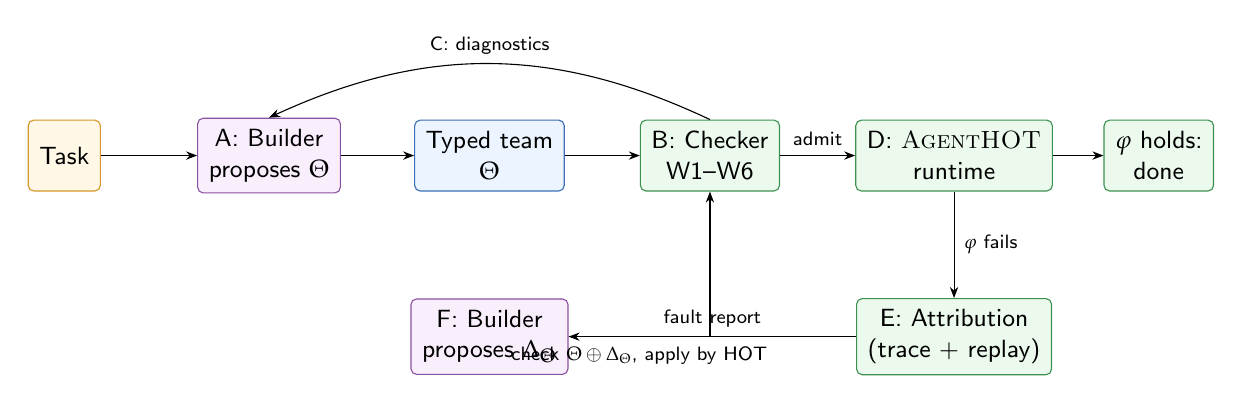
\begin{tikzpicture}[
  font=\sffamily\small, >={Stealth[length=4pt]},
  raw/.style={draw=rawbar, fill=rawbg, rounded corners=2pt, align=center, minimum height=9mm, inner sep=4pt},
  llm/.style={draw=llmbar, fill=llmbg, rounded corners=2pt, align=center, minimum height=9mm, inner sep=4pt},
  eng/.style={draw=enginebar, fill=enginebg, rounded corners=2pt, align=center, minimum height=9mm, inner sep=4pt},
  mod/.style={draw=modelbar, fill=modelbg, rounded corners=2pt, align=center, minimum height=9mm, inner sep=4pt},
  lbl/.style={font=\sffamily\scriptsize, align=center}]
  \node[raw] (task) at (0,0) {Task};
  \node[llm] (build) at (2.6,0) {A: Builder\\proposes $\Team$};
  \node[mod] (team) at (5.4,0) {Typed team\\$\Team$};
  \node[eng] (check) at (8.2,0) {B: Checker\\\W{1}--\W{6}};
  \node[eng] (run) at (11.3,0) {D: \tool{}\\runtime};
  \node[eng] (done) at (13.9,0) {$\varphi$ holds:\\done};
  \node[eng] (attr) at (11.3,-2.3) {E: Attribution\\(trace + replay)};
  \node[llm] (delta) at (5.4,-2.3) {F: Builder\\proposes $\Delta_\Team$};
  \draw[->] (task) -- (build); \draw[->] (build) -- (team); \draw[->] (team) -- (check);
  \draw[->] (check) -- node[above, lbl] {admit} (run);
  \draw[->] (run) -- (done);
  \draw[->] (check.north) to[bend right=25] node[above, lbl] {C: diagnostics} (build.north);
  \draw[->] (run) -- node[right, lbl] {$\varphi$ fails} (attr);
  \draw[->] (attr) -- node[above, lbl] {fault report} (delta);
  \draw[->] (delta) -| node[pos=0.25, below, lbl] {check $\Team\oplus\Delta_\Team$, apply by HOT} (check);
\end{tikzpicture}
\caption{\auto{}. LLM steps (purple) propose; deterministic steps (green)
decide. A team is executed only after the checker admits it, and every
repair passes the same checker.}
\label{fig:pipeline}
\end{figure}

\subsection{Step A: the builder proposes a typed team}\label{sec:typed}

A free-form builder outputs role prompts (\Cref{lst:captain}). An \auto{}
builder outputs a \emph{typed team}: the \tool{} team model extended with
what the checker needs.

\paragraph{Definition (typed team)} A typed team is a tuple
$\Team=(A,V,\mathbf{T},\omega,\kappa,\tau,G,\varphi)$ where
$A$ is a set of agents, each with a free-text role prompt (how it
\emph{thinks} remains prose);
$V=\{\MM_0,\dots,\MM_n\}$ is a set of view metamodels, $\MM_0$ being the
\emph{goal view} into which the task is lifted;
$\mathbf{T}$ is a set of hand-offs, each with source views
$\mathit{src}(T)\subseteq V$, one target view $\mathit{tgt}(T)$, and a set
of hybrid rules;
$\omega:A\to 2^V$ gives write rights;
$\kappa:A\to 2^{\mathit{Tools}}$ gives each agent's tools (code execution,
web search, \ldots);
$\tau$ maps each stochastic binding to the tools its prompt and validator
need;
$G$ is a set of \emph{goal obligations}, pairs $(C,s)$ of a goal-view class
$C$ and a scope predicate $s$ (``every accepted criterion'');
and $\varphi$ is an acceptance predicate built from engine-checkable
clauses only.

\plain{instead of handing us a stack of job descriptions, the builder must
hand us a blueprint: who the agents are, which form each one fills in,
which rules connect the forms, which tools each agent has, which goals must
be met, and how ``done'' is decided.}

\Cref{lst:proposal} shows a first proposal that a builder might make for
the \devteam{} task. It is \emph{illustrative}: we wrote it by hand to
contain one instance of each defect, so that the following steps have
something to find. It is a rendering of the file
\file{teams/devteam_proposal.json} that the reference checker reads.

\begin{lstlisting}[style=model, caption={Illustrative first proposal of a typed team for the \devteam{} task, containing one instance of each defect \D{1}--\D{5} (rendering of \file{teams/devteam_proposal.json}).}, label={lst:proposal}]
agents:   Analyst {tools: []}   Architect {tools: []}
          Developer {tools: [exec]}   Tester {tools: []}            -- D5
writes:   Analyst: Req   Architect: Arch   Developer: Code, Test     -- D3
          Tester: Test
goal:     (Criterion, c.story.status = 'accepted')
handoffs: Req2Arch  : Req  -> Arch  rules Story2Operation
          Arch2Code : Arch -> Code  rules Op2Edit
          Code2Test : Code -> Test  rules Edit2TestRun        -- D1: no rule reads Criterion
rule Story2Operation { from s : Req!UserStory (s.status = 'accepted')
   to op : Arch!Operation ( name <- s.title,
      signature <- @llm('Derive an API signature', s.title)    -- criteria not in footprint
      @check parses [form] ) }
rule Op2Edit { from op : Arch!Operation to e : Code!CodeEdit (
      file <- op.name,  operation <- op,
      body <- @llm('Implement', Sequence{op.signature, op.returnType}),  -- D2
      @check compiles [form] ) }
rule Edit2TestRun { from e : Code!CodeEdit to r : Test!TestRun (
      name <- e.file,
      verdict <- @llm('Run and judge', e.body) @check runs [behaviour, needs exec] ) }
done:     cover(G), valid, fresh, noObl, Tester.says('ALL TESTS PASS')    -- D4
\end{lstlisting}

\paragraph{Can an LLM write a typed team?} This is the premise of Step A, and
the MDE literature is cautious about it. LLMs asked to produce domain models
reach useful but imperfect accuracy~\cite{chen2023domainmodeling}, and
few-shot model completion helps but does not remove
errors~\cite{chaaben2023fewshot}; prompting itself can be
model-driven~\cite{clariso2023mdpe}. We draw two consequences. First, the
builder should not write free ATL and OCL: it fills a constrained format
(the JSON schema of our reference checker), in which footprints are
navigation paths and validators are chosen from a library with declared
strength and tool needs. Second, imperfect proposals are exactly what a
checker is for: a proposal that violates a condition is returned with a
diagnostic, not executed. How often a builder reaches an admissible team,
and in how many rounds, is a measured outcome of RQ2, not an assumption.

\subsection{Step B: the checker admits or rejects the team}\label{sec:check}

The checker evaluates six well-formedness conditions. Each is stated
first in plain words, then precisely, followed by the defect it rules out.
All six are evaluated on the team specification alone: no task data, no
LLM call, no execution. Several use the \emph{type-level dependency graph}
$\mathcal{G}_\Team$, whose nodes are the classes of all views and which has
an edge $C\to D$ for every rule whose source pattern contains $C$ and whose
target pattern creates $D$. A class $D$ is \emph{checked} if some rule
creating $D$ has a stochastic binding whose validator is executable (an
oracle, a parser, a compiler), written $\mathit{checked}(D)$.

\paragraph{\W{1}: Hand-offs are well typed} \emph{Every rule reads only
what its source forms contain and writes only what its target form
declares.} For every hand-off $T$ and rule $r\in T$: the source pattern's
classes belong to $\mathit{src}(T)$ and the target pattern's to
$\mathit{tgt}(T)$; every binding \code{f <- e} names a feature \code{f} of
its target class, and the static type of \code{e} conforms to the type of
\code{f}; every path in a footprint expression type-checks against
$\mathit{src}(T)$; stochastic bindings target primitive attributes only;
and every stochastic binding has a validator. \emph{Rules out the formal
part of \D{2}}: in \Cref{lst:proposal}, \code{op.returnType} does not exist
in \cls{Arch}, so the Developer's LLM would be prompted with information no
one produces.

\paragraph{\W{2}: Every artefact has exactly one writer} \emph{No two
agents write the same form, every non-goal form has an owner, and every
kind of object is created by one rule only.} The sets $\omega(a)$ are
pairwise disjoint and cover $V\setminus\{\MM_0\}$; for every class $D$, at
most one hand-off creates instances of $D$, and within it at most one rule.
(This is conservative: rules with provably disjoint guards could share a
target class.) \emph{Rules out \D{3}}: in \Cref{lst:proposal}, Developer
and Tester both write \cls{Test}.

\paragraph{\W{3}: Targets are complete} \emph{Every object a rule creates
gets all its mandatory fields, and every link it makes points to something
that exists.} For every rule $r$ creating $D$, each feature of $D$ with
lower bound $\ge 1$ is bound by exactly one binding of $r$; and every
structural binding that yields source objects of class $C$ for a reference
of type $D'$ is \emph{resolvable}, i.e.\ some rule maps $C$ to $D'$, so
that ATL's resolution finds a target. \emph{Rules out the content part of
\D{2}}: no consumer receives an object with an empty mandatory slot or a
dangling link.

\paragraph{\W{4}: Every obligation reaches a check that reads it}
\emph{Every goal the task states must flow, through the hand-offs, into a
value that a behavioural validator checks; and every agent's form must lie
on such a flow.} A path in $\mathcal{G}_\Team$ is not enough: a builder can
create one test case per criterion whose oracle never sees the criterion.
We therefore use the \emph{feature-level data-flow graph}
$\mathcal{F}_\Team$, with an edge $(C,f)\to(D,g)$ whenever a binding that
writes feature $g$ of target class $D$ reads feature $f$ of class $C$ in
its expression or footprint (a navigation path such as
\code{s.criteria.text} reads \code{UserStory.criteria} and
\code{Criterion.text}). Validators carry a \emph{strength}: \emph{form}
(parses, compiles, conforms to a schema) or \emph{behaviour} (executes the
value against an oracle or test). Let $B$ be the set of features written
by stochastic bindings with an executable behavioural validator. Then
\W{4} requires (a) for every goal obligation $(C,s)\in G$, some feature of
$C$ reaches $B$ in $\mathcal{F}_\Team$ (\emph{anchored coverage}); and
(b) every view is reachable from $\MM_0$ in the hand-off graph and reaches
a view containing a feature of $B$ (no idle or unverified agent).
\emph{Rules out \D{1}}: in \Cref{lst:proposal}, no binding reads any
feature of \cls{Criterion}, so no criterion ever influences a checked
value.

Two limits are explicit. \emph{Guards} on the rules along an obligation's
flow may exclude in-scope objects; whether they do is not decidable for
arbitrary OCL, so the checker emits a \emph{warning} for every guard that
differs syntactically from the obligation's scope, and the runtime clause
$\mathit{cover}(G)$ enforces coverage instance by instance. And anchored
coverage is relative to $G$: an obligation the goal view does not declare
is not checked. \Cref{sec:checkerstudy} shows a case in which this matters
and how declaring deliverables as obligations closes it.

\paragraph{Worked example: running \W{4} by hand} Let us compute
anchored coverage for the goal ``every accepted \cls{Criterion}'' in two
teams. Each arrow in \Cref{fig:w4} comes from one footprint or formula: an
arrow from \code{Criterion.text} to \code{TestCase.oracle} exists because
rule \code{Criterion2TestCase} gives the LLM \code{c.text} when it writes the
oracle. Green nodes are values checked by a \emph{behavioural} validator.

\begin{figure}[!htb]
\centering
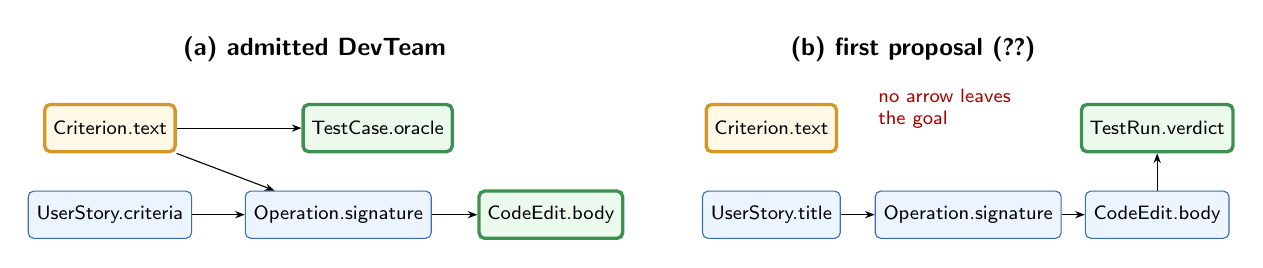
\begin{tikzpicture}[font=\sffamily\scriptsize, >={Stealth[length=3.5pt]},
  f/.style={draw=modelbar, fill=modelbg, rounded corners=2pt, minimum height=6mm, inner sep=3pt},
  b/.style={draw=enginebar, fill=enginebg, rounded corners=2pt, minimum height=6mm, inner sep=3pt, very thick},
  g/.style={draw=rawbar, fill=rawbg, rounded corners=2pt, minimum height=6mm, inner sep=3pt, very thick}]
  \node[font=\sffamily\small\bfseries] at (2.6,1.0) {(a) admitted \devteam{}};
  \node[g] (ct) at (0,0) {Criterion.text};
  \node[f] (sc) at (0,-1.1) {UserStory.criteria};
  \node[f] (sig) at (2.9,-1.1) {Operation.signature};
  \node[b] (body) at (5.6,-1.1) {CodeEdit.body};
  \node[b] (or) at (3.4,0) {TestCase.oracle};
  \draw[->] (ct) -- (or); \draw[->] (ct) -- (sig); \draw[->] (sc) -- (sig); \draw[->] (sig) -- (body);
  \node[font=\sffamily\small\bfseries] at (10.2,1.0) {(b) first proposal (\Cref{lst:proposal})};
  \node[g] (ct2) at (8.4,0) {Criterion.text};
  \node[f] (st2) at (8.4,-1.1) {UserStory.title};
  \node[f] (sig2) at (10.9,-1.1) {Operation.signature};
  \node[f] (body2) at (13.3,-1.1) {CodeEdit.body};
  \node[b] (ver2) at (13.3,0) {TestRun.verdict};
  \draw[->] (st2) -- (sig2); \draw[->] (sig2) -- (body2); \draw[->] (body2) -- (ver2);
  \node[text=red!65!black, align=left] at (10.6,0.25) {no arrow leaves\\the goal};
\end{tikzpicture}
\caption{Data-flow graphs for \W{4}. Orange: the goal's data. Green: values
checked by a behavioural validator. In (a) the goal reaches two green
nodes, so \W{4} passes. In (b) nothing ever reads \code{Criterion.text}, so
\W{4} fails, even though the team does test \emph{something}.}
\label{fig:w4}
\end{figure}

Start at the goal's data, here \code{Criterion.text}, and follow arrows. In
(a) you reach \code{TestCase.oracle} in one step: a test is written from
each criterion's text and must fail on a stub, a behavioural check.
\W{4} passes. In (b) there is no arrow out of \code{Criterion.text} at all;
the Architect wrote signatures from story titles only. The team still runs
code and judges verdicts, but none of that work ever saw a criterion, so
\W{4} fails. Notice why a path-only rule would be fooled: had the builder
added a rule that creates one empty test per criterion, a \emph{path} from
\cls{Criterion} to a checked class would exist, but there would still be no
\emph{arrow from the criterion's data}.

\paragraph{\W{5}: The engine decides completion} \emph{``Done'' is made of
things the engine can check, never of what an agent says.} $\varphi$ is a
conjunction of clauses from a fixed vocabulary: $\mathit{cover}(G)$ (every
goal object in scope has a validated descendant), $\mathit{valid}$ (all
validators pass), $\mathit{fresh}$ (no stale stamp), $\mathit{noObl}$ (no
open obligation or escalation); and the view graph is acyclic or declared
for the conservative scheduling strategy of Klare and
Gleitze~\cite{klare2023termination}. \emph{Rules out \D{4}}: the clause
\code{Tester.says(...)} in \Cref{lst:proposal} is not in the vocabulary.

\paragraph{\W{6}: Work goes to agents that can do it} \emph{An agent is
given an LLM-written value only if it has the tools that value's prompt and
validator need.} For every stochastic binding $b$ in a hand-off $T$ owned
by agent $a$ (i.e.\ $\mathit{tgt}(T)\in\omega(a)$),
$\tau(b)\subseteq\kappa(a)$. \emph{Rules out \D{5}}: \code{verdict.runs()}
needs code execution, which the Tester lacks.

\begin{think}
Without looking back: which condition rejects each of these teams?
(a) The Tester must run code but has no code-running tool.
(b) The Developer and the Tester both write test cases.
(c) ``Done'' is when the Tester says ``all tests pass''.
(d) No rule ever reads the acceptance criteria.
\end{think}

\paragraph{Assumed transformation fragment} The conditions assume
the declarative fragment of ATL that \tool{} uses: matched rules only (no
lazy, called or imperative rules); bindings whose expressions are
navigation paths or literals; footprints that are sets of navigation paths;
multi-source hand-offs matched over the disjoint union of their source
views; and validators drawn from a library that declares their strength and
tool needs.

\begin{remark}[Proposition 1: cost]
Each of \W{1}--\W{6} is decidable on the team specification in time
polynomial in its size $|\Team|$ (classes, features, rules, bindings and
path segments). \emph{Sketch.} \W{1} navigates each path once against the
metamodels; \W{2}, \W{3} and \W{6} count bindings and producers and compare
finite sets; \W{4}(a) is reachability in $\mathcal{F}_\Team$, whose size is
bounded by the number of path segments times the number of bindings;
\W{4}(b) and the cycle test of \W{5} are reachability and depth-first
search on the hand-off graph. No step needs task data or an LLM call.
\Cref{sec:checkerstudy} measures the reference implementation.
\end{remark}

\begin{remark}[Proposition 2: what admission guarantees]
Let $\Team$ be admitted and let the \tool{} runtime stop with $\varphi$
true. Then (i) every object in scope of a goal obligation is matched by a
rule chain that ends in a value whose behavioural validator passed and
whose footprint reads data derived from that object; (ii) no object has
two producing rules and no view two writers; (iii) every LLM-written value
was produced from a recorded footprint, under a stamp, and passed its
validator; and (iv) completion was decided by engine clauses only.
\emph{Sketch.} (i) $\mathit{cover}(G)$ in $\varphi$ requires, per object,
a validated descendant along a chain whose existence at type level
\W{4}(a) guarantees and whose instantiation ATL's matched-rule semantics
provides when guards admit the object; (ii) is \W{2}; (iii) is \W{1} with
the \tool{} runtime; (iv) is \W{5}.
\emph{Not guaranteed:} that the metamodels capture what the task needs,
that validators are strong enough, or that agents reason well. A
well-typed team can still go wrong; it can go wrong in fewer, and more
diagnosable, ways.
\end{remark}

\plain{Proposition~1 says the checker is fast because every rule is a
simple count, a set comparison or a ``can I get from here to there''
question. Proposition~2 says what a passing team promises: every goal is
tested by something that actually read it, nothing is written twice,
every LLM answer passed a check, and only the engine says ``done''. It does
not promise the agents are clever.}

\subsection{Step C: diagnostics drive the builder's repair}

When a condition fails, the checker returns a \emph{diagnostic}: the
condition, the offending element, and enough context to fix it.
Diagnostics are fed back to the builder, which proposes a revised team; the
loop is bounded by $k_{\mathit{adm}}$ rounds. \Cref{lst:diag} is the
reference checker's actual output on \Cref{lst:proposal}: one violation per
seeded defect, and no other.

\begin{lstlisting}[style=engine, caption={Output of the reference checker \file{teamcheck.py} on \file{teams/devteam_proposal.json}.}, label={lst:diag}]
W1  Op2Edit.body: footprint path 'op.returnType': Arch!Operation has no feature 'returnType'
W2  view Test written by ['Developer', 'Tester']; needs exactly one writer
W4  goal obligation (Criterion, c.story.status = 'accepted'): no behavioural
    validator reads data derived from Criterion
W5  done-clause Tester.says('ALL TESTS PASS') is not engine-checkable
W6  Edit2TestRun.verdict needs ['exec']; owner Tester has []
REJECTED: 5 violation(s)
\end{lstlisting}

Diagnostics differ from an LLM critic's comments in two ways. They are
\emph{complete} for the conditions checked: a team that passes has none of
these violations, whereas a critic may miss one. And they are
\emph{actionable at the right granularity}: they name a rule, a footprint
path or a write right, not ``improve coordination''.

\subsection{Step D: the admitted team runs on \tool{}}

An admitted team runs on the unchanged \tool{} runtime: deterministic rule
structure, stochastic bindings over footprints with validators and up to $k$
samples, persisted trace models with version stamps, obligations under
change, and the engine-decided acceptance predicate.

\subsection{Step E: attribution by construction}\label{sec:attrib}

If $\varphi$ does not hold when the runtime stops, the engine knows which
clauses fail and, through the trace models, where.

\what{Locate.} A failed $\mathit{cover}(G)$ clause names a goal object with
no validated descendant and the first rule on its path that did not fire:
a composition fault at a named place. A failed $\mathit{valid}$ clause, or
an escalation, names one pair $(t,b)$: a target object, one stochastic
binding, the rule and hand-off that contain it, the agent that owns it, and
the stamped footprint the LLM saw. Attribution to agent and hand-off is
therefore a lookup, not an inference over a transcript.

\what{Classify.} Locating the binding does not yet say \emph{why} it failed.
Because the footprint is recorded and small, the engine can replay the
binding cheaply, which TraceElephant found useful for transcripts as
well~\cite{chen2026traceelephant}:
\begin{enumerate}
\item \emph{Replay} $b$ on its stamped footprint $r$ more times. If some
sample passes, classify as a \textbf{sampling fault}: the composition was
adequate and this agent's LLM was unlucky or too weak (remedy: retry, or
give the owner a stronger model).
\item Otherwise \emph{widen} the footprint by one hop and replay. For a
rule with source variables $x_1,\dots,x_m$, widening adds every path
$x_i.f$ for each feature $f$ of $x_i$'s class and every path $x_i.r.g$ for
each reference $r$ and each attribute $g$ of $r$'s target class; for a
multi-source hand-off this ranges over all source variables. If a sample now passes, classify as a \textbf{footprint
fault}: the hand-off did not carry what the consumer needs, an instance of
\D{2} (remedy: widen the footprint in the team).
\item Otherwise inspect the footprint's values. If one of them was itself
written by an upstream stochastic binding, classify as an \textbf{upstream
candidate} and repeat the procedure on that binding, following the trace
model backwards.
\item Otherwise classify as a \textbf{specification fault}: the prompt or the
validator cannot be satisfied by any value the footprint supports (remedy:
revise the binding's prompt or validator).
\end{enumerate}
The procedure assumes deterministic validators. Before classifying, the
engine runs the failing validator twice on the same value; if the verdicts
differ, it reports a \textbf{validator fault} (for example, a test that
depends on the network) instead of blaming any agent. The procedure makes
at most $2r$ LLM calls per binding visited and visits at
most as many bindings as the longest path in $\mathcal{G}_\Team$. The
classification is a heuristic; whether it agrees with ground truth is part
of RQ3.

\subsection{Step F: checked re-composition}

A fault report goes back to the builder, which proposes a \emph{team delta}
$\Delta_\Team$: widen a footprint, add a rule, add an agent and its form,
move a binding, strengthen a validator. The checker evaluates
$\Team\oplus\Delta_\Team$ exactly as in Step~B; only an admitted delta is
applied, as a higher-order transformation over the running team model, as
in \tool{}. Because accepted values carry stamps, the delta creates
obligations only where it changes a footprint or a rule; values elsewhere
are kept. Rebuilding the team from scratch, as a free-form builder must,
discards them.

\begin{center}
\begin{minipage}{0.92\linewidth}
\begin{tcolorbox}[enhanced, colback=white, colframe=black!25, arc=0pt, boxrule=0.5pt,
  left=6pt, right=6pt, top=4pt, bottom=4pt, title={\sffamily\small Algorithm 1: the \auto{} loop}, 
  coltitle=black, colbacktitle=black!6, fonttitle=\bfseries]
\small
\begin{tabbing}
\quad\=\quad\=\quad\=\kill
\textbf{input} task $x$; budgets $k_{\mathit{adm}}$ (admission), $k_{\mathit{rep}}$ (repairs), $r$ (replays)\\
$\Team \gets \textsc{Propose}(x)$;\ \ $i\gets 0$ \hfill \textit{Step A}\\
\textbf{while} $\textsc{Check}(\Team)=\mathit{diag}\neq\emptyset$ \textbf{and} $i<k_{\mathit{adm}}$:\ \ $\Team\gets\textsc{Revise}(\Team,\mathit{diag})$; $i\gets i+1$ \hfill \textit{Steps B, C}\\
\textbf{if} $\mathit{diag}\neq\emptyset$ \textbf{then return} \textsc{NotAdmitted}($\mathit{diag}$)\\
\textbf{for} $j=0,\dots,k_{\mathit{rep}}$:\\
\>$(\mathit{ok},\mathit{fails})\gets\textsc{RunAgentHOT}(\Team)$ \hfill \textit{Step D}\\
\>\textbf{if} $\mathit{ok}$ \textbf{then return} \textsc{Done}\\
\>$\mathit{report}\gets\textsc{Attribute}(\mathit{fails},r)$ \hfill \textit{Step E}\\
\>$\Delta\gets\textsc{ProposeDelta}(\Team,\mathit{report})$;\ \textbf{if} $\textsc{Check}(\Team\oplus\Delta)=\emptyset$ \textbf{then} $\Team\gets\textsc{ApplyHOT}(\Team,\Delta)$ \hfill \textit{Step F}\\
\textbf{return} \textsc{Failed}($\mathit{report}$)
\end{tabbing}
\end{tcolorbox}
\end{minipage}
\end{center}
\phantomsection\label{alg:auto}
{\small Only \textsc{Propose}, \textsc{Revise}, \textsc{ProposeDelta} and the
bindings inside \textsc{RunAgentHOT} call an LLM; admission, execution
structure, attribution lookup and completion are deterministic.}


\begin{think}[Check your understanding: attribution]
A binding fails its validator three times. On replay with the same
footprint it passes once in five tries. Which fault class does \auto{}
report, and what remedy does that suggest?
\end{think}

\subsection{What \auto{} does not solve}\label{sec:limits-design}

\begin{itemize}
\item \textbf{Adequacy of the forms.} The checker verifies that the team
fits together, not that its forms capture what the task needs. A builder
can propose a well-typed team whose metamodels omit an essential concept;
the omission becomes a \D{1} defect only if the goal view states the
concept as an obligation. \textsc{Lift}, which turns the task text into the
goal view, remains a free-text boundary, as in \tool{}.
\item \textbf{Validator strength.} \W{4} requires an executable validator on
every path; it cannot require a \emph{good} one. Weak validators turn
content errors into accepted values.
\item \textbf{Reasoning errors.} Failures inside one agent's reasoning (MAST
FM-1.1, 2.2, 2.6) are outside any composition check; \auto{} can at best
classify them as sampling or specification faults.
\item \textbf{Expressiveness.} Teams whose value lies in open-ended dialogue,
such as debates, do not decompose naturally into forms and rules. RQ2
measures what typing costs on tasks where such teams help.
\end{itemize}

\begin{takeaway}
\begin{itemize}
\item \auto{} splits team building the way \tool{} splits hand-offs: an LLM
\emph{proposes}, a deterministic program \emph{decides}.
\item Six rules (\W{1}--\W{6}) check the blueprint before anything runs; each
rules out one kind of defect from \Cref{tab:defects}.
\item When a run fails anyway, trace records point to one value of one
hand-off, and a cheap replay suggests whether the agent, the hand-off, an
upstream value or the specification is to blame.
\item Repairs are checked by the same six rules before they are applied.
\end{itemize}
\end{takeaway}
% ===========================================================================
\section{A first look at the checker}\label{sec:checkerstudy}
% ===========================================================================

Before the studies of \Cref{sec:plan}, we implemented the six conditions
to see whether they can be implemented as stated, what they catch, and
what they cost. This section reports that implementation. Its results
concern the checker, not task success.

\subsection{Setup}

The reference checker \file{teamcheck.py} is about 300 lines of Python
without dependencies. It reads a typed team in JSON and prints diagnostics
(\Cref{lst:diag}). We wrote four typed teams. \file{devteam_proposal} is
the seeded proposal of \Cref{lst:proposal}; \file{devteam_admitted} is a
corrected \devteam{}. \file{chakin_pilot} is our encoding of the
hand-written team of the \tool{} pilot on DevBench \texttt{chakin}, as
described in the \tool{} companion document: hand-offs \code{Req2Arch},
\code{Arch2Code} and \code{Req2Test}, a \code{parses} validator on
signatures, a \code{compiles} validator on code bodies, and an oracle
validator on test cases. \file{chakin_repaired} applies one delta to it
(below).

\subsection{Finding 1: the seeded proposal yields exactly the seeded defects}

On \Cref{lst:proposal}, the checker reports five violations, one per
seeded defect, and nothing else (\Cref{lst:diag}).

\subsection{Finding 2: the hand-written pilot team is rejected}

\begin{lstlisting}[style=engine, caption={Checker output on \file{teams/chakin_pilot.json}, our encoding of the hand-written \tool{} pilot team.}, label={lst:pilot}]
W4  view Arch reaches no behavioural check (its work is never verified)
W4  view Code reaches no behavioural check (its work is never verified)
REJECTED: 2 violation(s)
\end{lstlisting}

The team that the \tool{} pilot ran by hand is \emph{not} admitted
(\Cref{lst:pilot}). Its code bodies are checked only for compiling, and no
hand-off feeds code into a behavioural check; criteria are tested, but the
tests never run against the code. The \tool{} reports describe the same
weakness informally: its validators checked form, not meaning, a
\code{compiles()} check accepted a function that ignored its criterion, and
no configuration passed DevBench's acceptance tests~\cite{agenthot2026}.
The checker turns that observation into a named violation at a named place.
One delta, replacing the body's validator by a behavioural one that
executes the criteria's oracles (and needs the code-execution tool the
Developer has), makes the team admissible. Whether that delta would raise
DevBench acceptance is a question for RQ2, not something the checker can
show.

\subsection{Finding 3: mutation study}

We wrote one or two mutation operators per defect class and applied each
at every applicable site of the two admitted teams, giving 82 mutants
(\Cref{tab:mutants}). To test whether \W{4} needs anchoring, we ran
every mutant twice: with \emph{anchored} \W{4} as defined in
\Cref{sec:check}, and with a \emph{naive} \W{4} that only requires a
class-level path from each goal class to some class with an executable
validator. We also ran two goal configurations: $G_1$ declares only
acceptance criteria as obligations; $G_2$ also declares user stories, that
is, the deliverables.

\begin{table}[!htb]
\centering\small
\caption{Mutation study on \file{devteam_admitted} and \file{chakin_repaired}
(82 mutants). Cells: mutants detected (any violation). All results are
reproduced by \file{mutate.py}. The unmutated teams produce no violation
in any configuration.}
\label{tab:mutants}
\begin{tabular}{@{}l l r r r r r@{}}
\toprule
& & & \multicolumn{2}{c}{$G_1$ = criteria} & \multicolumn{2}{c}{$G_2$ = criteria + stories} \\
\cmidrule(lr){4-5}\cmidrule(l){6-7}
Defect & Mutation operator & Mutants & anchored & naive & anchored & naive \\
\midrule
\D{1} & delete a rule & 7 & 6 & 6 & \textbf{7} & 7 \\
\D{1} & detach goal data from all footprints & 2 & \textbf{2} & 0 & \textbf{2} & 0 \\
\D{2} & break a footprint path & 8 & 8 & 8 & 8 & 8 \\
\D{2} & drop a mandatory binding & 20 & 20 & 20 & 20 & 20 \\
\D{3} & add a second writer to a view & 18 & 18 & 18 & 18 & 18 \\
\D{3} & duplicate a producing rule & 7 & 7 & 7 & 7 & 7 \\
\D{4} & add an agent's claim to $\varphi$ & 8 & 8 & 8 & 8 & 8 \\
\D{4} & drop an engine clause from $\varphi$ & 8 & 8 & 8 & 8 & 8 \\
\D{5} & remove a required tool & 4 & 4 & 4 & 4 & 4 \\
\midrule
& Total & 82 & 81 & 79 & \textbf{82} & 80 \\
\bottomrule
\end{tabular}
\end{table}

Three observations stand out.

\what{Path-based coverage has a blind spot.} The ``detach'' operator keeps
every rule but removes, from every footprint, each path that reads goal
data, so that test cases still exist per criterion but their oracles never
see the criterion. Naive \W{4} accepts both detached teams; anchored \W{4}
rejects both. A coverage check that looks only at which kinds of objects
are created would admit a team that tests nothing it was asked to test.

\what{Coverage is relative to the declared goal.} Under $G_1$, one mutant
escapes all six conditions: deleting \code{Story2Operation} from the
\texttt{chakin} team. The result is a team that writes and validates a
test for every criterion but never creates an operation or any code: every
declared obligation still reaches a behavioural check. Declaring the
deliverable as an obligation ($G_2$) catches it. The lesson for builders
is concrete: the goal view must declare what is to be \emph{delivered},
not only what is to be \emph{checked}.

\what{Violations name the right condition.} In 81 of the 82 detections
under $G_2$, the condition the operator targets is among those reported.
The remaining one, deleting \code{Epic2Component}, is reported under
\W{3}: operations still refer to their epic, whose component is now never
created, which is a dangling reference and therefore a hand-off mismatch,
as it should be.

\subsection{Finding 4: cost}

On synthetic chain teams of $n$ views with one hand-off between
consecutive views, the reference checker took 0.5\,ms for $n=10$,
5\,ms for $n=100$, 0.21\,s for $n=1{,}000$ and 1.8\,s for $n=3{,}000$
(single core, Python 3.12). Teams built by today's builders have between
one and five agents (\Cref{tab:audit} and~\cite{chen2026traceelephant}),
so checking costs far less than a single LLM call and can run on every
candidate inside a builder's search loop.

\subsection{What this does and does not show}

The study shows that the six conditions are implementable as defined, that
anchoring and declared deliverables are necessary for \W{4} to mean what
it says, and that checking is cheap. It does not show that real builders
can emit admissible typed teams, that admitted teams fail less, or that
violations correspond to the failures of real runs. The mutation operators
are ours and target our own conditions, so high detection is expected by
construction; its value lies in the two blind spots it exposed and in the
exact location of each diagnostic. The \texttt{chakin} encoding is ours,
from a published description. These limits are the reason for RQ1--RQ3.

\begin{think}
Why is it not impressive, on its own, that the checker kills mutants
designed by the same authors for the same rules? What \emph{is} informative
about \Cref{tab:mutants}?
\end{think}

\begin{takeaway}
\begin{itemize}
\item The six rules can be implemented in about 300 lines and run in well
under a second on realistic teams.
\item A coverage rule that only asks ``is there a path?'' is fooled; the rule
must ask ``does a real check \emph{read} the goal?''.
\item Coverage is only as good as the goals you declare: declare what must be
\emph{delivered}, not just what must be \emph{tested}.
\end{itemize}
\end{takeaway}
% ===========================================================================
\section{How each research question will be answered}\label{sec:plan}
% ===========================================================================

\subsection{Subjects shared by all three studies}

\paragraph{Team builders} Four builders that span the design space of
\Cref{tab:builders}: CaptainAgent~\cite{song2024captain} (per-step team
building), AutoAgents~\cite{chen2024autoagents} (team plus plan, observer
critique), MetaAgent~\cite{zhang2025metaagent} (explicit control states)
and MAS-Zero~\cite{ke2025maszero} (per-instance design with LLM
meta-feedback). All are open source.

\paragraph{Tasks} General-assistant tasks from GAIA and AssistantBench, to
connect with Who\&When~\cite{zhang2025whowhen}, and software-engineering
tasks: the Python repositories of DevBench~\cite{li2024devbench}, whose
PRDs, UML diagrams and executable tests the \tool{} pilot already
uses~\cite{agenthot2026}.

\paragraph{Models} At least two model families, one open-weight, at fixed
temperature, five seeds per task and configuration; all builders and
agents in one configuration use the same model.

\subsection{RQ1: diagnosis}\label{sec:plan-rq1}

\what{Data.} (a) The 184 annotated failures of Who\&When, whose 126
algorithm-generated cases come with their team specifications; (b) new
failing runs of the four builders on the tasks above, logged with full
inputs as TraceElephant recommends~\cite{chen2026traceelephant}.

\what{Procedure.} We extend the audit of \Cref{sec:audit} to every builder
(specification-level evidence). For causal evidence, two coders
independently label each failure with its decisive cause: one of
\D{1}--\D{5}, \emph{agent reasoning}, \emph{tool/environment}, or
\emph{other}, using a codebook with definitions and examples from
\Cref{tab:defects}. They start from the existing Who\&When annotation (agent,
step, reason) and decide whether the composition caused it. Agreement is
reported as Cohen's $\kappa$ on a first round; disagreements are resolved
by discussion. A third coder re-codes a 20\% sample.

\what{Measures.} Share of failures whose decisive cause is a composition
defect, with 95\% bootstrap confidence intervals, per defect, builder and
task family; agreement with the analytical mapping of \Cref{tab:defects}.

\what{Refutation.} We set the threshold below the share of the smallest
of MAST's three categories (task verification, 23.5\%~\cite{cemri2025mast}):
if composition defects explain less than any single MAST category, they
are not a major cause. If the lower bound of the confidence interval for
the composition share is below 20\% on both task families, we will report that
the composition gap, although present in specifications, is not a major
cause of failure, and re-scope RQ2 to attribution only.

\subsection{RQ2: prevention}\label{sec:plan-rq2}

\what{Conditions.} For each builder: \textbf{Free} (as published);
\textbf{Critic} (as published plus an LLM critic that reviews the team for
\D{1}--\D{5}, the strongest non-deterministic alternative); \textbf{Schema}
(agents exchange JSON validated against one shared schema, in the style of
PatchBoard~\cite{zhang2026patchboard}); and \textbf{\auto{}} (the builder is
prompted to emit a typed team; checker and repair loop as in
Algorithm~1).

\what{Static measures.} A mutation analysis on admitted typed teams: one
mutation operator per defect (delete a rule on a goal path, \D{1}; break a
footprint path or drop a mandatory binding, \D{2}; duplicate a write right
or a producing rule, \D{3}; add an agent-claim clause to $\varphi$, \D{4};
remove a required tool, \D{5}). For each condition we report detection
rate and false-alarm rate (rejections of unmutated teams). For the
\textbf{Critic} condition, the same mutants are rendered as prose.

\what{Dynamic measures.} Task success (GAIA/AssistantBench answers; DevBench
unit and acceptance tests); composition-caused failures per 100 runs, coded
as in RQ1; admission rounds; tokens and wall-clock for building and running;
and the share of tasks for which no admissible team was found within
$k_{\mathit{adm}}$ rounds (the cost of typing).

\what{Hypotheses and refutation.} H2a: the checker detects all mutants of
the classes it targets, with no false alarms on admitted teams; this is
expected by construction, \Cref{sec:checkerstudy} confirms it on two
hand-written teams under $G_2$, and RQ2 repeats it on builder-generated
teams. H2b:
\auto{} has fewer composition-caused failures than Free, Critic and Schema.
H2c: task success under \auto{} is not lower than under Free. If H2b holds
but H2c fails, typing prevents defects at too high a cost in
expressiveness; if H2b fails, the checker's conditions do not capture the
defects that matter, which RQ1's codes will show.

\subsection{RQ3: attribution and repair}\label{sec:plan-rq3}

\what{Ground truth.} Faults injected into runs of admitted teams, one
class at a time: a wrong value accepted by a weak validator upstream
(upstream), a footprint made one hop too narrow (footprint), an
unsatisfiable validator (specification), and a temperature or model
downgrade on one agent (sampling); plus natural failures coded as in RQ1.

\what{Baselines.} The transcript-based attribution methods of
Who\&When (all-at-once, step-by-step, binary search)~\cite{zhang2025whowhen}
and an agentic attribution method with replay as in
TraceElephant~\cite{chen2026traceelephant}, applied to the same runs
rendered as transcripts with full inputs.

\what{Measures.} Agent-level and binding-level (step-level) accuracy;
accuracy of the fault class; LLM calls spent on attribution. For repair:
success after one checked delta, tokens spent, and the number of accepted
values preserved, compared with rebuilding the team from scratch.

\what{Hypotheses and refutation.} H3a: location by trace lookup is exact
for injected faults (by construction; a miss indicates an implementation
error). H3b: fault classification agrees with ground truth more often than
the best baseline's reason labels. H3c: checked repair succeeds at least as
often as rebuilding and costs fewer tokens. If H3b fails, the replay
procedure is not a reliable classifier, and \auto{}'s attribution reduces
to exact location without diagnosis.

\subsection{Threats to validity}\label{sec:threats}

\what{Selection.} Who\&When contains only failed runs. The audit therefore
describes failing teams' specifications and how their failures ended; it
cannot compare them with succeeding teams. RQ1's new runs include
successes, so that specification properties can be compared between
succeeding and failing teams.

\what{Construct.} The defect codes are ours; we mitigate with a codebook,
two independent coders and $\kappa$, and we publish all codes. Mutation
operators are designed by us for our own defect classes, so H2a and H3a
measure implementation correctness, not discovery; H2b and H3b carry the
claims. The audit of \Cref{sec:audit} is lexical: it can miss interfaces
stated in unusual wording. We inspected every match and publish the
patterns.

\what{Internal.} A builder prompted to emit typed teams may differ in
quality from the published builder for reasons unrelated to checking. We
include a condition in which the builder emits a typed team that is
executed \emph{without} the checker, to separate the effect of the format
from the effect of the check.

\what{External.} Four builders, two task families and two model families
do not cover the field. Who\&When's teams come from one builder; this is
why RQ1 adds new runs. Software-engineering tasks are limited to Python
DevBench repositories.

\what{Conclusion.} Five seeds per configuration and bootstrap intervals;
paired comparisons per task with Wilcoxon signed-rank tests and effect
sizes.

\begin{takeaway}
\begin{itemize}
\item RQ1 measures how often the composition, not an agent, causes failure;
RQ2 asks whether checking blueprints prevents that; RQ3 asks whether trace
records find and fix failures better than reading transcripts.
\item Each question says in advance which result would prove us wrong.
\end{itemize}
\end{takeaway}

% ===========================================================================
\section{Related work}\label{sec:related}
% ===========================================================================

\paragraph{Automatic construction of agent teams} \Cref{sec:ev-builders}
reviewed builders that generate roles, plans, state machines or workflow
code~\cite{song2024captain,chen2024autoagents,chen2024agentverse,liu2024dylan,yuan2025evoagent,zhang2025metaagent,ke2025maszero,hu2025adas,zhang2025aflow,zhang2025maas,zhuge2024gptswarm,qian2025macnet,he2026tpgo}.
\auto{} is complementary: it does not propose a new search strategy but a
target representation that any of them could emit, and a check that any of
them could run inside its loop.

\paragraph{Learned orchestration} A fast-growing line trains an
orchestrator with reinforcement learning to choose agents, sub-tasks and
communication~\cite{dang2025puppeteer,nielsen2026conductor,ke2026masorchestra},
or evolves agent graphs and topologies~\cite{yang2025agentnet,zhang2025gdesigner,ma2026ann}.
These systems learn \emph{which} team to build; \auto{} would let them check
\emph{whether} a proposed team fits before spending reward on running it.
We also conjecture, without evidence yet, that the checker's diagnostics
could give such learners a richer training signal than a single task
reward; testing this is future work. Studies
of how teams behave, such as expert under-use~\cite{pappu2026experts}, the
communication--reasoning gap~\cite{zhang2026silobench}, collaboration
benchmarks~\cite{zhu2025multiagentbench} and emergent
coordination~\cite{riedl2026emergent}, motivate checks that do not rely on
coordination emerging by itself.

\paragraph{Failure analysis and attribution} MAST, the edge-level
taxonomy of AgentAsk, Who\&When and TraceElephant characterise and
attribute failures from
transcripts~\cite{cemri2025mast,lin2026agentask,zhang2025whowhen,chen2026traceelephant}.
AgentAsk intervenes at hand-offs with learned clarification
questions~\cite{lin2026agentask}. \auto{} attacks the same hand-offs
statically, and makes attribution a lookup plus a bounded replay.

\paragraph{Structured communication} MetaGPT's structured documents,
schema-validated shared state, DSPy's typed signatures for LM pipelines,
Agora's negotiated protocol documents, and MCP/A2A make individual messages
well-formed or transport them
reliably~\cite{hong2024metagpt,zhang2026patchboard,khattab2024dspy,marro2024agora,mcp2024,a2a2025}.
They check messages; \auto{} checks the \emph{team}: coverage, single
writers, completeness, termination and capabilities across all hand-offs.

\paragraph{Software architecture and agent-oriented SE} Architectural
mismatch, contracts and connector specifications motivate our
conditions~\cite{garlan1995mismatch,garlan2009mismatch,meyer1992dbc,allen1997connection};
Gaia's role schemas anticipated write permissions and
protocols~\cite{wooldridge2000gaia}. The difference is who composes: an
LLM, per task, without a human review.

\paragraph{Model-driven engineering} \auto{} reuses ATL's execution model
and static typing~\cite{jouault2008atl}, persisted
traceability~\cite{jouault2005traceability,vara2014metagem}, incremental
execution~\cite{jouault2010incremental}, HOTs~\cite{tisi2009hot},
models@run.time~\cite{blair2009runtime}, and termination strategies for
transformation networks~\cite{stevens2020networks,klare2023termination}.
Its MDE contribution is a set of well-formedness conditions for
transformation networks whose authors are LLMs and whose values are
stochastic. Work on LLM-generated domain models and model
completion~\cite{chen2023domainmodeling,chaaben2023fewshot,clariso2023mdpe}
studies the quality of individual generated models; \auto{} checks how
generated models and transformations fit together.

% ===========================================================================
\section{Conclusion}\label{sec:conclusion}
% ===========================================================================

Automatically assembled teams of LLM agents are assembled the way software
was assembled before interfaces: from parts described by what they are good
at, not by what they require and provide. Published failure studies, the
difficulty of attributing those failures, and our audit of 126 generated
teams all point to the composition as a major, unchecked source of failure.
\auto{} asks team builders for something a machine can check, a typed team,
and keeps the LLM where it is strong: proposing teams, prompts and values.
A reference checker already rejects a hand-written team for a weakness its
authors had only described, and exposes two blind spots that a naive
coverage check would have. Three research questions, each with a
refutation criterion, will tell us how much of the gap this closes in
practice.

\paragraph{Data availability} The anonymous artifact contains the audit
script and its output (\file{audit_whowhen.py}), the reference checker
(\file{teamcheck.py}), the six typed teams (\file{teams/*.json}), the
mutation and scaling scripts with their outputs (\file{mutate.py},
\file{scale.py}), and the RQ1 codebook; the \tool{} prototype on which \auto{} builds is available as
described in~\cite{agenthot2026}.

\appendix
% ===========================================================================
\section{Reproducing the audit}\label{app:repro}
% ===========================================================================

\begin{lstlisting}[language=bash, style=engine]
git clone https://github.com/ag2ai/Agents_Failure_Attribution     # commit f4d2b6d
W="Agents_Failure_Attribution/Who&When"
python audit_whowhen.py "$W/Algorithm-Generated" "$W/Hand-Crafted"   # Tables 3, 4
python teamcheck.py teams/devteam_proposal.json                     # Listing 5
python teamcheck.py teams/chakin_pilot.json                         # Listing 6
python mutate.py teams/devteam_admitted.json teams/chakin_repaired.json          # Table 8, G1
python mutate.py teams/devteam_admitted_g2.json teams/chakin_repaired_g2.json    # Table 8, G2
python scale.py                                                     # Finding 4
\end{lstlisting}

The script reads, for each of the 126 files, the generated role prompts
(\code{system_prompt}), the first message of the run (the manager's brief,
with its plan and output format), the annotated mistake agent, and the
messages that contain \code{TERMINATE}. Teammate names are matched with word
boundaries, so that \code{Food_Expert} does not match inside
\code{Vegan_Food_Expert}. Every match of every pattern was inspected by
hand; the patterns are in the script.

% ===========================================================================
\section{Glossary}\label{app:glossary}
% ===========================================================================

\begin{description}[leftmargin=1.2em, style=nextline, itemsep=1pt]
\item[Agent] An LLM in a loop with tools and a role (\Cref{sec:course}).
\item[ATL] A rule-based language for model-to-model transformations~\cite{jouault2008atl}.
\item[GAIA, AssistantBench, DevBench] Public benchmarks of tasks for agents; DevBench contains small software projects with their tests.
\item[GNN] Graph neural network: a learned model that reads and produces graphs.
\item[LLM] Large language model: a non-deterministic text predictor.
\item[MAST] A published taxonomy of 14 ways multi-agent LLM systems fail~\cite{cemri2025mast}.
\item[OCL] The expression language for navigating models; \code{s.criteria.text} reads like Java field access.
\item[Oracle] An automatic judge of whether an output is correct, such as an assertion in a test.
\item[RL] Reinforcement learning: learning by trial and numerical reward.
\item[Who\&When] A public dataset of failed multi-agent runs, annotated with the agent and step responsible~\cite{zhang2025whowhen}.
\item[Anchored coverage] Condition \W{4}: some feature of each goal object flows into a value that a behavioural validator checks.
\item[Architectural mismatch] Parts that work alone fail together because of hidden assumptions about each other~\cite{garlan1995mismatch}.
\item[Binding (structural / stochastic)] How a field of a created object gets its value: by a formula, or by an LLM that sees only its footprint.
\item[Composition gap] Team members have no checked interfaces, so nothing verifies that they fit (\Cref{sec:plain}).
\item[Footprint] The exact source data an LLM may read when writing one value.
\item[Hand-off] One agent's output becoming another agent's input.
\item[HOT] Higher-order transformation: a transformation that produces a transformation, used to change a running team.
\item[Metamodel / model] A form (schema) and a filled-in form (data that conforms to it).
\item[Mutation testing] Evaluating a checker by planting mistakes (mutants) and counting how many it catches (kills).
\item[Obligation] A value whose inputs changed and must be redone; also, in $G$, a goal that must be met.
\item[Team builder] A system that designs an agent team automatically for each task.
\item[Trace link] A record that a target object was created from a source object by a rule.
\item[Typed team] A team blueprint the checker can read: agents, forms, rules, write rights, tools, goals, and the definition of ``done''.
\item[Validator (form / behaviour)] A check a value must pass: ``does it parse?'' versus ``does it pass the tests?''.
\end{description}

% ===========================================================================
\section{Answers to the questions in the orange boxes}\label{app:answers}
% ===========================================================================

\what{Interfaces (\Cref{sec:course}).} There is no interface: the Developer
reads an English message and guesses. Nobody checks it.

\what{Shared chat (\Cref{sec:audit}).} A shared chat shows everyone the same
words, but it does not say \emph{who owns} each step, \emph{what form} a
result must take, or \emph{who decides} that the work is finished.

\what{Change to \code{S2.1} (\Cref{sec:background}).} The signature of
\code{S2}'s operation, the oracle of \code{S2.1}'s test, and \code{S2}'s code
body, because their footprints contain \code{S2.1}'s text (directly or through
the signature). \code{S1}'s operation reads only \code{S1}'s data, so its
stamp is unchanged.

\what{Which condition (\Cref{sec:check}).} (a) \W{6}; (b) \W{2}; (c) \W{5};
(d) \W{4}.

\what{Attribution (\Cref{sec:attrib}).} A sampling fault: the hand-off gave
the agent enough information, and the LLM simply failed most of the time.
Remedy: retry, or give that agent a stronger model.

\what{Mutation study (\Cref{sec:checkerstudy}).} Because the mutants were
designed to break exactly the rules the checker enforces, catching them
mainly shows the code is correct. What is informative is what the study
\emph{exposed}: that a path-only coverage rule misses ``detached'' teams,
and that one mutant escapes unless deliverables are declared as goals.

\bibliographystyle{ieeetr}
\bibliography{autom2m-references}

\end{document}